% REMEMBER: You must not plagiarise anything in your report. Be extremely careful.

\documentclass{l4proj}

    
%
% put any additional packages here
%

\begin{document}

%==============================================================================
%% METADATA
\title{Level 4 Project - Virtual Turing Tumble}
\author{Luke Gall, 2298070g}
\date{September 14, 2018}

\maketitle

%==============================================================================
%% ABSTRACT
\begin{abstract}
    Every abstract follows a similar pattern. Motivate; set aims; describe work; explain results.
    \vskip 0.5em
    ``XYZ is bad. This project investigated ABC to determine if it was better. 
    ABC used XXX and YYY to implement ZZZ. This is particularly interesting as XXX and YYY have
    never been used together. It was found that  
    ABC was 20\% better than XYZ, though it caused rabies in half of subjects.''
\end{abstract}

%==============================================================================

% EDUCATION REUSE CONSENT FORM
% If you consent to your project being shown to future students for educational purposes
% then insert your name and the date below to  sign the education use form that appears in the front of the document. 
% You must explicitly give consent if you wish to do so.
% If you sign, your project may be included in the Hall of Fame if it scores particularly highly.
%
% Please note that you are under no obligation to sign 
% this declaration, but doing so would help future students.
%
\def\consentname {Luke Gall} % your full name
\def\consentdate {20 March 2020} % the date you agree
%
\educationalconsent


%==============================================================================
\tableofcontents

%==============================================================================
%% Notes on formatting
%==============================================================================
% The first page, abstract and table of contents are numbered using Roman numerals and are not
% included in the page count. 
%
% From now on pages are numbered
% using Arabic numerals. Therefore, immediately after the first call to \chapter we need the call
% \pagenumbering{arabic} and this should be called once only in the document. 
%
% Do not alter the bibliography style.
%
% The first Chapter should then be on page 1. You are allowed 40 pages for a 40 credit project and 30 pages for a 
% 20 credit report. This includes everything numbered in Arabic numerals (excluding front matter) up
% to but excluding the appendices and bibliography.
%
% You must not alter text size (it is currently 10pt) or alter margins or spacing.
%
%
%==================================================================================================================================
%
% IMPORTANT
% The chapter headings here are **suggestions**. You don't have to follow this model if
% it doesn't fit your project. Every project should have an introduction and conclusion,
% however. 
%
%==================================================================================================================================
\chapter{Introduction}

% reset page numbering. Don't remove this!
\pagenumbering{arabic} 


Why should the reader care about what are you doing and what are you actually doing?
\section{Guidance}

\textbf{Motivate} first, then state the general problem clearly. 

\section{Writing guidance}
\subsection{Who is the reader?}

This is the key question for any writing. Your reader:

\begin{itemize}
    \item
    is a trained computer scientist: \emph{don't explain basics}.
    \item
    has limited time: \emph{keep on topic}.
    \item
    has no idea why anyone would want to do this: \emph{motivate clearly}
    \item
    might not know \emph{anything} about your project in particular:
    \emph{explain your project}.
    \item
    but might know precise details and check them: \emph{be precise and
    strive for accuracy.}
    \item
    doesn't know or care about you: \emph{personal discussions are
    irrelevant}.
\end{itemize}

Remember, you will be marked by your supervisor and one or more members
of staff. You might also have your project read by a prize-awarding
committee or possibly a future employer. Bear that in mind.

\subsection{References and style guides}
There are many style guides on good English writing. You don't need to
read these, but they will improve how you write.

\begin{itemize}
    \item
    \emph{How to write a great research paper} \cite{Pey17} (\textbf{recommended}, even though you aren't writing a research paper)
    \item
    \emph{How to Write with Style} \cite{Von80}. Short and easy to read. Available online.
    \item
    \emph{Style: The Basics of Clarity and Grace} \cite{Wil09} A very popular modern English style guide.
    \item
    \emph{Politics and the English Language} \cite{Orw68}  A famous essay on effective, clear writing in English.
    \item
    \emph{The Elements of Style} \cite{StrWhi07} Outdated, and American, but a classic.
    \item
    \emph{The Sense of Style} \cite{Pin15} Excellent, though quite in-depth.
\end{itemize}

\subsubsection{Citation styles}

\begin{itemize}
\item If you are referring to a reference as a noun, then cite it as: ``\citet{Orw68} discusses the role of language in political thought.''
\item If you are referring implicitly to references, use: ``There are many good books on writing \citep{Orw68, Wil09, Pin15}.''
\end{itemize}

There is a complete guide on good citation practice by Peter Coxhead available here: \url{http://www.cs.bham.ac.uk/~pxc/refs/index.html}. 
If you are unsure about how to cite online sources, please see this guide: \url{https://student.unsw.edu.au/how-do-i-cite-electronic-sources}.

\subsection{Plagiarism warning}

\begin{highlight_title}{WARNING}
    
    If you include material from other sources without full and correct attribution, you are commiting plagiarism. The penalties for plagiarism are severe.
    Quote any included text and cite it correctly. Cite all images, figures, etc. clearly in the caption of the figure.
\end{highlight_title}


%==================================================================================================================================
\chapter{Background}
What did other people do, and how is it relevant to what you want to do?
\section{Guidance}
\begin{itemize}    
    \item
      Don't give a laundry list of references.
    \item
      Tie everything you say to your problem.
    \item
      Present an argument.
    \item Think critically; weigh up the contribution of the background and put it in context.    
    \item
      \textbf{Don't write a tutorial}; provide background and cite
      references for further information.
\end{itemize}


If I wanted this to focus more for school children. I could try and either target high school or primary and if so maybe talk to the teachers there?

Each puzzle in the starting book has a start set up and a list of available parts they could use, solutions are also given, so puzzles and the right output could be tracked in an app?


% This is where I should put any notes when researching the turing tumble or any virtual comterparts
Turing Tumble is a marble game that can build mechanical computers using various components and gears
Can help teach people how simple switches work which act as the building block to computers. Can teach logic gates, truth tables, conditionals, binary etc

The online version they recommended is very much just the game, could look at making it more of an edu tool by having the puzzles available online and maybe making my own?
Depends if I want it to be used in class rooms for school children in schools where they won't want to get the physical boards due to practice

The balls act as the electricity going through the board

The game board has two flippers, one that releases the blue ball and one that releases the red ones
6 different parts
Ramp directs balls left or right depending on which way it is put in, this moves a ball along the vertical track. These are like wires in normal computing terms
Crossover lets ball paths cross over, so can cross paths that some balls may have. Crossover acts as 2 wires crossing over each other, but not touching
bit, points left or right storing logic. These act as switches which allow the balls to change the course of the next set of electricity 

Interceptor stops any more balls being released, if the ball stops, 'electricity' stops meaning it no longer runs
Gears and gear bits are the components that help make the board turing complete, the bit part stores logic 

Gears and gear bits let other gear bits to turn each other. Can turn gear bits above, side or below them. Needs to be used in combination with gears as they aren't weighted correctly overwise
By using gears we can send info back up the board, so we could send up to the top that a register is above a certain number i.e. for loops
Different combinations of gear bits and bits made different logical pieces, like the latch which lets one blue left and the rest right (2 gear bits top left and bottom with a gear)
Set switch lets you make all bits point in a certain direction, lets you test the direction (bit value) without changing it
Can make a flip flop using gear and gear bits to remember info about it before it drops

This switch can be used to check overflow etc. The combinations that gears and gear bit could be made to do could be explored?


Features that can be improved upon with virtual one online, no save Elements, no login etc. Could be useful? Could encourage people to make puzzles online? 
\emph{Notes on Java Swing}
For java swing, intellij has a swing Ui designer which can be used to automatically add different components to the app without needing to code from scratch
Has a main JFrame which will seems to act as the main desktop app panel that buttons, etc can be placed in. 
Hovering over the components in Intellj doesn't give too much information into what they actually do are why we need them. Could be someone to focus on improving.

The Java swing API has it's main super class as a Component (Object is above this like every java class). It can then be a Container or JComponent. Where a container is either a window or a panel, and the 
components are labels, lists, tables etc. 

Swing isn't really designed for animations, java fx is recommended instead


\emph{Angular vs React} 
Angular is made and maintained by Google using the Typescript as it's main language

React is a front end JS lib for building UI interfaces, made by facebook. More interaction based way of working with the UI Elements

React uses a virtual DOM so would be quicker to re-write elements of HTML Doc (Could include the board pieces)
Angular uses a real DOM so it needs to update the entire HTML tree even for little changes

React is smaller and therefore faster to load up

I already have a bit of knowledge of angular so it might be easier to start with

matter js could be used, plus also animejs and angular has it's own animation library

\emph{React notes}
These notes were taken while undertaking the official react tutorial

Mainly about composing complex UIs from lots of components which are smaller and more singular pieces of code
React will re update and render the components if the data changes.

Reach component class takes in prop and returns a react Element
Can put any JS expressions inside the JSX, so could be a different react class (say a component for the turing tumble)

Parent components can pass data down to child Elements using props, don't think it can go the other way 
Components have state. State can be considered private 

Children props can pass state to each other using shared state stored in the parent component. Parent component can pass the state back down to the children by using props
Keeps the child components in sync

In the tutorial we push state up from the lower down child component so it gets state from it's parent and uses the function provided by it. Making it a controlled component
The tutorial recommends always keeping state immutable and replacing this with new objects instead of changing the existing state for error handling and the ability to check changes more easily in the future
Helps the react engine know when it should update it's rendering 

\emph{Angular vs React vs Vue} 
Frameworks don't equal library's. Libs are pre written code with classes, functions etc, can download these from npm or github
Frameworks include a large stack of functions and help the dev use the various features that would otherwise need to be made before the real site can be done, i.e. routing etc

React is only the UI library would need other technologies to handle any backend (if needed) for example
Vue can let you use JS or Typescipt, but Angular's documentation is all in Typescript but can use normal JS or Dart if needed. 
This makes it good for devs form OO background tho. Angular forces the three file approach to a component while react and vue don't
React is one way binding only which may be an issue. 

\emph{Angular notes} 

I know a little bit of angular already so it wouldn't be a complete deep dive into web dev and could probably help save some hours.
It is fully component based, the components are the main building tools for the framework, each component consists of Typescript, html and css files 
Components are organised hierarchy, this will help force a good layout for my code and will help encourage good practices 
Can support data flow from component to the template - property
    template to the component - event
Can two way bind using these, using a fairly complex background of watchers
Got a slightly steeper learning curve by all accounts 
Typescript is pretty similar to Java or C

\emph{p5}

p5 could be used as a drawing library but I would need to spend some more time looking at it

\emph{Matter js notes (https://brm.io/matter-js/)}
It is a 2D physics engine for shapes and objects, that could be useful to model the marbles going down the slope of the game board
Matter js has an internal engine that updates the animations for us

engine has a timescale object which will slow down animations, which could be useful
x, y starts from top left.
This is a very powerful library with some very interesting examples on their site, this could be a very powerful tool to use to make the envo but it may be difficult to apply the logic of the balls and components, may be easier to 
focus on the logic then add some animation?

Engine is the module for creating and maintains the physics engine while render is the module that visualizes the objects moving
World module is used to provide methods and props to create and manipulate the world, i.e. gravity
Bodies is circles rectangles and other common solid Bodies
body is used to manipulate properties of bodies ie density, velocity etc
Composites allow a quick creation of multiple bodies like a stack of rectangles 

It would definitely be possible to create turing tumble using this library it might just be too powerful for what we need 

% SHOULD MAYBE LOOK AT WCAG
\emph{Online board games}
Tabletop simulator is the most popular game that allows people to play board games in a 3d desktop game that allows multiple people to play 'physical' like online board games.
The player can touch, pick up and move objects which can interact with the board game. Can be a bit complicated for new users however and is very reliant on learning the controls and 
playing the game 'physically'. There is a large mod scene for this game which allows new games and versions to be added by fans of the game creating a large ecosystem of different games for people to play.
The rules for board games need to enforced by the players, it is more a sandbox for the game pieces to exist in which users will manipulate them like in real life to follow the play of the game.
This is the more 'hardcore' version for people serious about playing 3d versions of board games with great community made games and lots of mod-ability.

This game is on the game platform Steam, it also contains a lot of separate virtual versions of popular board games that can be purchased separately which have various levels of polish and online aspects.
Including a GoT board game or versions of Monopoly.

In terms of browser based online board games there is Boardgame Arena which is free online but offers paid exclusive content including better UI or more popular
games. Only the host is required to have the premium games that allows friends to play them together with other people that have the free version. Unlike tabletop simulator
the rules are enforced and it includes tooltips to ensure people can understand the rules as they play the game. It has a fairly simple look and feel to the board games
by using only a top down 2d view on the board. Which makes it easier on slower computers but doesn't make it the most visually appealing. 
Focusing more on logic instead of look and feel while keeping the game 2d will make it more accessible to a wider audience while reducing load on slower PCs.

Many educational games exist online aimed at providing a family friendly and fun way for kids to learn and have fun. Some are made by large charities including Animal Jam made by NatGeo. 
Tinybob has a wide variety of online games aimed at teaching children different subjects. The visuals are very applying and there is a great sense of style and attention put into the games, leading to many awards for the company 
and it's various games. Including ones learning the body, simple physics, the Earth and some Mammals. If I was to go down a more kid focused educational route
these games would be ones to look at.

%==================================================================================================================================
\chapter{Analysis/Requirements}

% Talk about how the requirements were split into reqs needed be to be meet to match existing projects and then the reqs added to imrpove upon these projects 


% Talk about adding puzzles as the external motivator to encourage people to use the app, therefore increasing the possiblit that it could be useful in a learning concept

The main aim of this project was to create a virtual simulation of a Turing Tumble board game. As stated in the background multiple versions of the game exist online so one of the major requirements was to include new features to distinguish this program from existing implementations. A minor requirement was to create a program that could be used in a classroom environment where it could be used to encourage the use of this program to help teach logical skills useful in a Computer Science context. The problem was researched by studying the Turing Tumble board game and the existing simulations that exist online to develop a set of functional and non-functional requirements that would meat the brief. user evaluation was carried out by university students and school pupils undertaking a computer science course to gain valuable insight into new features that could be added and improvements that can be implemented to better meet the non-functional requirements.

\section{Requirements}
To meet the main aim as described above a list of major functional requirements are listed below with their MoSCoW (REF) prioritization tier, these are described below. As the main aim of the project is well understood and has been demonstrated by various existing programs the major requirement that had to be researched was to distinguish this program from these versions with a feature that could be seen as unique enough to help separate this implementation from the existing programs and be useful in helping users learn more about the Turing Tumble. It was decided that by adding puzzle creation and playing as a requirement it could meet both of these requirements. The idea was inspired from the physical board game that comes with a set of puzzles to help teach children how to use the board including it's various pieces and is designed to teach them about different physical components that exist within computer circuits. 

The following list of requirements uses the MoSCoW prioritization method to distinguish which features were most important within the scope of the project. 
\begin{itemize}
    \item Must Have (\textbf{M}) - The set of requirements needed to meet the minimum viable program that can meet the brief.
    \item Should Have (\textbf{S}) - The set of requirements that should be focused on to add value to the program without it's success wholly reliant on it.
    \item Could Have (\textbf{C}) - A desirable extra requirement that shouldn't affect the existing project if not achieved.
    \item Would Like (\textbf{W}) - A requirement that won't be delivered due to the scope of the project but are stated for future work considerations.
\end{itemize}

\textbf{Functional Requirements}
\begin{itemize}
    \item (M) Allow users to view, place, and delete pieces on a virtual Turing Tumble board. This should include the 6 pieces present within the physical Turing Tumble as well as the two slot types they are placed in. This will allow a user to build any pattern possible on the physical Turing Tumble.
    \item (M) Allow users to simulate a valid board. This allows users to play through a Turing Tumble board and understand how the various pieces influence a passing marble.
    \item (M) correctly simulate the Gearbit and Gear pieces. These two pieces are required to add Turing completeness to the Turing Tumble and should be able to interact with other connected Gearbits. This will allow the user to create more complicated boards and puzzles.
    \item (M) Add playback features to a board. Including a pause / play, speed slider and a step forward feature. This will allow the user to play the pace at their preferred pace helping them understand the exact path a marble takes on the board.
    \item (M) Ensure pieces match the logic present in the physical Turing Tumble. The pieces placed by the user should directly match the logic of the pieces in the physical game. This allows the boards created by a user to directly simulate a board created on the physical game.
    \item (M) Marbles should be clear and visible on the board. This includes the amount of marbles in the 2 coloured marble dispensers, the marble in play, and the collected marbles at the bottom of the board. This will allow the user to directly view where the marble is during its execution as well as aid understanding on the path it will take. Collected marbles are required to understand the output of the Turing Tumble and allow pattern to be created by the board.
    \item (M) Allow users to edit the number of marbles present in the default board. This will allow users to change how many marbles could be released by the board.
    \item (M) Allow users to play puzzles. This includes adding the main descriptors required to understand what the puzzle is about, including a title, description, hwo many pieces the user has available, and it's expected output. This will allow a user to learn more about the Turing Tumble while providing a fun way to learn more about logic needed in Computer Science.
    \item (M) Allow users to create puzzles. This will allow users to create new puzzles that other users can play, creating an ecosystem of puzzles that can be played over time improving overall learning using the game.
    \item (S) Clearly display where a piece can be placed. Will help aid in understanding of how to place the pieces onto the board while improving understand of the rules of the game. 
    \item (S) Allow users to save and upload boards. This will users to create patterns then save them for future visits to the site.
    \item (S) Users should be able to login to the site. This will allow the site to monitor which user created the puzzle and display the author name on created puzzles. 
    \item (S) Have a list of default puzzles created for users to work through. A list of puzzles should be uploaded to the site so users have a set to play through without needing the online puzzle ecosystem to be very active.
    \item (S) Create a tutorial page to describe the game and the application. This should allow a user to understand how the application works and how the Turing Tumble game plays.
    \item (S) Create a home page. Should give an brief overview to the site and the different pages a user can access.
    \item (C) Allow users filter through puzzles using a difficulty filter. This will give the user greater control of which puzzles they see and allow a greater ease of learning by giving the option to start with more simpler puzzles before moving onto more complicated ones.
    \item (C) Add a description to each piece to increase understandability. This will greater improve the usability of the pieces and allow users to learn how the piece works without needing to check the tutorial page. 
    \item (C) A user should be able to change the theme of the program. This will add accessible to the site and allow the user to choose a theme they prefer.
    \item (C) Add a selection of example board configurations to show more complicated patterns and functionality of the board. For example an addition pattern could be added to show how the Turing Tumble can use Bit pieces to add two binary numbers together.
    \item (C) Allow users to comment and rate other puzzles. This will help create a more active puzzle environment were users can encourage each other to create more elaborate puzzles that others can enjoy.
    \item (W) A user page were users can delete or edit there published puzzles. This will encourage users to create puzzles and update older puzzles with any possible fixes or edits to improve the puzzle for other users.
    \item (W) Full gravity simulation for the board. This would greatly improve the visual appeal of the game and be a very faithful recreation of the physical game. It would also add to user enjoyment, encouraging greater use of the site and possible learning effects.
    \item (W) A leaderboard where users completion time for puzzles can be views. This will give an extra environment aspect to complete puzzles for users. 
    \item (W) Allow a user to edit the size and dimensions of the board. This would allow users to create more complicated patterns and puzzles to fully simulate the computational power of the Turing Tumble. 
\end{itemize}

\textbf{Non-functional Requirements}
\begin{itemize}
    \item (M) No existing knowledge of a Turing Tumble should be required to understand and use the app. As this program is decided to introduce people to the Turing Tumble game, it must be easy to use for this target audience.
    \item (M) Should be intuitively from the outset without the need to keep going back to a tutorial to understand how to use it. After the first read of the tutorial which describes the game, the UI elements shouldn't need too much explanation and should be easy to understand.
    \item (M) Should be runnable on modern browsers with no software install required. This will allow school pupils and Computer Science students to use it without the need to install software, which may be unavailable for some.
    \item (C) Should be quick and efficient to use on most modern desktop devices. Users will be unlikely to return to a website if it is slow and inefficient, keeping the user experience as enjoyable as possible will increase the possible uptake of the site.
    \item (W) Should be runnable on mobile devices. Some users may not have access to a desktop or laptop so making sure the app can run on more common mobile devices could increase the number of users of the program.
\end{itemize}

\section{Specification updates}
The requirements was changed halfway through development time. The project was planned to go one of two way. It was either going to focus on full physics simulation to improve the user experience or puzzle playing and creation was going to be the focus. In both cases it was important to first ensure that the minimum viable product was created in which a Turing Tumble board could be successfully simulated. Time was then spent deciding which possible course of action would be the best given the remaining development time. Puzzles were chosen as the next major requirement in order to give a unique feature to the program that other online versions don't contain. After adding the puzzle features it was decided that development time was better focused on general improvements than adding full physics simulation. 

% Write up of Turing Tumble Pieces

\emph{Ramp} 
The Ramp component is the simplest component and acts as a 'wire' in the computer metaphor that persists throughout the components. 
The Ramp sends a ball either right or left depending on the direction the curved end is facing, the ramp doesn't care which way the ball enters
the component, it will send right / left for a ball entering from the top right or left of the component. This piece is reversible in order to change the direction
it faces. As the balls aren't allowed to drop freely until they reach the end, the ramp is the most common way to direct the balls to the desired location.
This components representation in code should store the direction it is facing which will be the direction it sends the ball or 'electricity' down.

\emph{Crossover}
The Crossover is a non reversible piece that continues the direction a ball is travelling into the component but allows the balls to enter from either side.
If a ball enters from the top left, travelling to the bottom right, it will leave the bottom right side of the crossover continuing it's direction. As this is a 
static piece, the crossover can't be reversed and will always act the same way. This piece is metaphorically equivalent to wires crossing over in chips, it allows paths created 
using ramps and other components to cross over each other.

\emph{Bit}
The Bit component acts as a metaphorical switch that will change the direction the next ball will travel based on if it is on (pointing to the right) or off (pointing to the left).
If the bit is pointing to the right (on) send the balls to the left no matter which direction they enter from. Send the balls to the right if the switch is pointing to the left (off).
However when a ball passes through a bit it changes the direction it is facing so it isn't a perfect analogy when comparing them to switches inside circuits. These components can be used to represent registers
that store bit values which can then be used to represent values in binary representation.
This component will need to store the direction it's facing as it's only main property.

\emph{Interceptor}
This component catches a ball and stops the execution of the turing tumble as the marble will no longer be able to reach the end of the board and release another marble. 
By using the metaphor of electricity this component stops the electricity from flowing through the computer meaning it will stop execution.
This component is similar to a shutoff switch inside a regular computer. It will not store any properties but should be able to change the position of the ball to static and 
stop the run time of the board.

\emph{Gear}
Gears are the only components that can be placed on pegs instead of slots on the board and act as connections between a number of gear bits. They turn either 90 left or right. They will need a turn function.

\emph{Gear Bit}
This component is a like a bit in that it stores state by pointing left or right and will send a ball in the opposite direction it is facing and then change direction.
A Gear Bit not connected to a Gear will act and behave exactly like a normal Bit component. When a gear bit changes direction it will also turn any connecting gears this direction which can 
then in turn change other gears and gear bits. The combination of this component and the gear makes the game Turing Complete. 
Information can only be sent down the board unless using these components which can then be used to affect components above the gear bit that gets switched.
This component like the bit will need to be able to store it's direction (state) and then turn itself and any connecting gears.

Using a combination of gear and gear bits we can make new logical components like latches, fixed position switches, set switches and flip flops. The logic of these
new composite components could be explored plus the creation of new components that provide different logic.
\section{Guidance}
Make it clear how you derived the constrained form of your problem via a clear and logical process. 

%==================================================================================================================================
\chapter{Design}
% Doesn't need to be in this order, just possible headings
\section{Application Logic}
\subsection{Component design and architecture}
One important design decision made from the onset was to focus on using a component design philosophy to group together related user facing UI code, backend functionality, and styling rules into modular Components that can be called in different locations and can be sent different input values to display different data to the user using the same repeated internal functionality code. This allows for example, a single component to represent the various board pieces, this component can then be given exact piece data and represent this as a view to the user but the component can abstract way the exact information of which piece it needs to display.

\subsection{Piece Interface}
An important objective of the design stage was to abstract away the logic of the individual board pieces so that the algorithm designed with looping through the boards main execution cycle of the marble going down the board wouldn't need to check the underlying functionality of the piece objects that interact with the marble. To meet this objective a Board Piece abstract class was created that contained various properties including the image locations of pieces, position of the piece, and it's tooltip. It was to also include abstract methods for processing a marble, which would change the direction of the marble based on the logic of the piece. This abstraction of the main logic for piece objects allowed the marbles to be more easily processed by the board.

\subsection{Board design}
A large design consideration involved the representation of a Turing Tumble board itself. It was decided that a class should be created to store all data related to the board as well as any methods required to update it's data that will be displayed to the user, for example the number of held blue marbles. It was an important idea to keep all data related to a board contained within a single object that ensured that no board related data could be edited without using its exported function calls. The main section of the board class that needed modeled was the slots that would contain the various board pieces. An interface design was chosen such that component slots and pin slots could be abstracted away to ensure that the slots could be separated into the two distinct types of slots without adding development overhead to the board class to identify which slot it was dealing with during execution. A 2 dimensional array representation was chosen for the various slots on the board. The board pattern of 11 by 11 slots (some of which are empty) lends naturally to the indexing properties of the array and as no extra slot will be added or replaced during execution, the speeds related to indexing the 2d array were seen as advantageous. 

\subsection{Collected Marbles}
The marbles collected by the board is the main output given to the user by the execution of the board. A class design that stored collected marbles into pairs of consecutively collected marbles of the same colour was designed. This allows a large list of marbles to be minimized into it's most important details to more compactly display data to the user, focusing on the details important to a Turing Tumble board, how many marbles of a certain colour were seen in a row. 

\subsection{Single In play marble}
One design decision that was made to reduce possible errors when dealing with the main looping function calculating the marble position was to ensure that only one marble could be in play at one time. This was to ensure that the board only had to calculate the logic of a single marble using it's slots instead of having extra overhead of working with multiple falling marbles. While in the physical board game a user can release multiple marbles at the same time, this is not encouraged and can lead to users ignoring the main learning objective of creating a path that a marble would flow down to flip the next marble, instead of releasing what ever marble was needed by the user.

\subsection{Playback options}
3 main playback options were designed for the board, play / pause, step forward and speed increase / decrease. As a Turing Tumble can be quite confusing for new users, a speed value was designed to be changed by the user so that they could find a speed comfortable for their ability. Pausing execution allows the user to stop the execution of the board to greater understand the processes involved before continuing board execution. A step forward function was designed that would pause execution then move the marble to it's next location, bypassing any speed constraint. This gives total control to a user in how quickly or slowly they wish to go through various parts of the board, allowing them to step forward the more trivial aspects or sped more carefully when interacting with a more complicated pattern. No step backwards function was designed as the development complexity of going back through the more complicated Turing compete Gearbits wasn't seen as a high priority. 

\subsection{Main execution algorithm}
The algorithm design responsible for calculating and updating the current position of the in play marble was designed by looping through a function responsible with calculating the next marble position. It checks that a marble is currently on the board and processes the marble using the piece that it is currently sharing a slot position with. If the marble is out of position it would be calculated if this position could trigger a new marble. It was decided that when a marble reached a slot that contained no piece it would be seen as an error and a user would need to release a new marble. This was to follow the rules set out by the physical Turing Tumble were users are discouraged from dropping marbles a great distance between multiple components, this would encourage users to skip complicated patterns in favour of dropping a marble to the bottom. Which in the physical board game can lead to physical damage to the board, it was therefore seen as a more faithful simulation if this feature was not allowed in this program. By having the main execution function not loop itself but merely update the marble using the individual pieces function it allowed for easier implementation of playback features, as functions could be created that would call this function with different interval speeds or pause execution and wait for the user to toggle the board to play this function again.

\subsection{Puzzle Board design}
One main feature that was designed was the implementation of puzzles for users to play. The design of the puzzles was chosen to follow the puzzle design from the official Turing Tumble board game. As the focus of this program is to simulate a Turing Tumble board faithfully the puzzles that come with the game were used as default puzzles for a user to play. The board was designed to extend the existing board class so the UI code could accept a puzzle board as data and still display the board to the user without development time spent updating existing UI components accepting this new object. Properties of this new class included the data required to store various states of a puzzle including the starting marbles a user has that can't be changed, the expected output that a user must try to achieve and how many pieces they have to do so. Another benefit of having this class extend the original board object was the reuse of existing code, all logic required to calculated the position of marbles was retained and only functions required to check new conditions were added. This included a new function to deal with the change in how users could add pieces to a board, during a puzzle a user only has a certain amount of pieces they can place while staying within the puzzle limits. This was added to ensure that users couldn't bend the set rules of the puzzles and add correction enforcement.   

\subsection{Puzzle creation design}
An important feature that was added to allow users to create their own puzzles for other users to play. The design of this feature followed the different aspects of a physical Turing Tumble puzzle that were required and how a user could create them. A phase system was created were users would use the existing board and placement features to create the different aspects of the puzzle. The first phase required the user to set up the board with the starting pieces for the puzzle that would be locked in place for a user. Once these pieces were confirmed the user enters the next phase were they are asked to create the solution to their puzzle, the creator then plays through this solution collecting the marbles they wish to be the final output before confirming this output. One issue was to design a possible checking feature that would ensure that any puzzle uploaded by a user would be possible to complete using the given available pieces and that the starting set up was a valid Turing Tumble board. To meet this requirement it was decided that by asking the user to place pieces on an existing board object all the logic related to ensuring that only valid pieces were placed was already present and could be used to ensure that a user couldn't create an invalid starting set up. By asking a user to create the solution and run through it's output before confirming, it forces users to create a valid solution to a possible puzzle so no puzzle can be uploaded with impossible output given the list of pieces available. This also allowed the users to create a puzzle using a system they were familiar with and removed the potentially challenging task of creating a Turing Tumble puzzle validator for a puzzle entered without checks. The final phase was a simple input form in which users are asked to name their puzzle, give a description of the object and assign its difficulty. These descriptive aspects were chosen from the puzzles given in the physical Turing Tumble game.

\subsection{Piece placement}
To allow users to place the pieces on the board, it was designed that a click and place feature would be implemented instead of the possibly more intuitive drag and drop. Click and place was chosen as it was seen to be more efficient for users after they learn how to use the feature. A Turing Tumble has 106 valid slots were pieces can be placed, click and place would be far more time efficient for users to place a large number of consecutive pieces of the same type. While drag and drop may be more intuitive initially it was decided that the time to drag and drop multiple pieces would be inefficient and demand too much time. To meet this click and place feature a selection bar was designed were a user could chose a piece, updating an internal value in the board object and then when a slot is clicked board would calculate if this piece was valid.


\subsection{Board Validity}
One area of design that needed attention was how to ensure that marbles would always be in a valid position on the board and couldn't be directed outwith the board area or towards invalid slots. This design followed naturally from the design of the physical Turing Tumble board, where the slot types form a criss cross pattern (PUT diagram). As the various pieces of the board will always send marbles down one level of the board and either one place to the left or right. A piece will always send a marble to another component slot that may or may not contain a piece. The only exception to this is the component slots on the far left or right of the board. In the physical board game walls are at both sides of the board, meaning a marble that is sent into the wall will drop to the pin slot below. This has been added in the design of the marble execution function but will lead to the marble falling and stopping execution.

\section{User Interface}
% Include wireframes that were made and why I choose the one I did
\subsection{Internal Consistency}
The user should find the program easy to use and once learned shouldn't have any difficulty navigating the site. To meet this the site was designed such that an internal consistency was present between the multiple pages. In this regard it was decided that all pages with a Turing Tumble board present would use the same board UI elements and have an identical selection bar placed to it's left. The theme between the various pages is kept constant with a global style specification, the theme was designed to be changed from light to dark to meet the users preference while still having a clear and accessible appearance. A top title bar was designed to be present in all pages with the change of page changing the main view window but leaving the top title bar and side navigation bar constant to keep consistency between the multiple pages.

\subsection{Board Design}
A wireframe was created for the main board design as shown in fig (REF), the design closely follows the design from the physical Turing Tumble, with the various slots placed a set distances from each other. Marble values were designed to be displayed as a single number at the top left and right corners to match the physical version were marbles are held in dispensers in the top two corners. A number was designed instead of a collection of images to allow for an quicker way to determine the number of marbles left while avoiding a large number of icons for larger marble values required for some patterns. The collected marbles were designed to follow the physical board by being displayed in the bottom right corner with the the most recently collected colour marble sequence on the left to follow the natural queue order present in the physical board.

\subsection{Page Design}
The main user interface for the plain board was designed after examining 2 other virtual Turing Tumbles. Some design decisions to consider from these pages include
\begin{itemize}
    \item The board should be the largest element and in the centre of the page.
    \item Pieces should be on the left and include it's icon.
    \item Options related to the board could be on the left or right of the board.
    \item Triggering the marbles could be placed under the board.
    \item Speed options could be a list of toggle.
\end{itemize}

After examining these pages 3 initial wireframes were created for possible page designs as shown in fig (REF). The wireframes were created online using draw.io (REF). Different design elements were considered in each with wireframe 3 ultimately being the main design that was improved on during the implementation stage. In all designs it was important to have emphasis placed on the board by placing it in the centre of the page with the largest visual footprint. Options were placed on either side or just the left but ultimately it was chosen that options should be placed on one side to allow for a greater sized board. A side navigation bar was chosen to reduce to visual impact of a top navigation bar and was designed with the idea to be able to hide and show the navigation when required. Focusing on keeping on the necessary options visible when possible allowing the greatest focus and impact for the board at any one time. It was designed that only options available to the user should be shown and that icons would be greyed out to signify that the option was unavailable leading to less visual weight to options not useful to the user at that certain time. By disabling buttons and having a clear UI to convey this it was designed that users would have a greater understanding of the boards state and not be tempted to press buttons with an illegal action.


\subsection{Piece Design}
The design of the pieces was chosen to closely mimic the physical board pieces. To match this, all pieces were given a distinct colour matching it's physical counterpart, keeping them easy to identify between each other. The pieces matched the colour of the physical pieces but it was decided that the exact physical appearance didn't need to exactly match the physical version this was because the physical version pieces need to include sections related to the pieces fitting on the board. It was decided to remove these sections of the appearance to focus more on the distinguishable parts of the piece design. For example the ramp component was designed to include just the sloping ramp instead of the coupling section needed to place the piece on the board.

\section{Technologies}
The following technologies were chosen to meet the specification and capture the functional requirements.

\subsection{Angular}
Angular was chosen as it is a full component based javascript (JS) framework with components split into modules of HTML, Typescript, CSS and a testing file. Typescript is a super script of JS adding static type checking (REF) and allows for greater control over the creation of classes and interfaces compared to base JS. The components in Angular are organised in a hierarchy and can help keep a strong modular implementation. Angular comes prepackaged with some very helpful libraries including a testing framework, routing service and forms. It is also very easy to add a wide variety of different JS libraries using Node Package Manager (NPM) allowing more development time spent on implementing the functionality instead of creating solving issues solved by external libraries. While this project is focused mainly with building a web application, Angular can be used to built native mobile applications so the implementation can made more portable as part of possible future work.

\subsection{Material UI}
Material UI created by Google was chosen as an external user interface library to add high quality UI elements to the application. Material UI components are highly reliable and already tested to ensure that UI in the program are easy to use and follow a standard seen elsewhere. Material UI components are added to existing code by using a call to an individual component using Angular notation and editing the component using its API.

\subsection{Web Application}
This program was designed to built as a web application. One reason was the goal to have this program be easily accessible to users so the high portability of a web application with easy access for many users with a desktop or laptop. Second is that the program was designed with user integration in mind so a web application lends itself naturally to storing user data in a backend server that can then be displayed to other users. Lastly a web application is more accessible for users in a classroom environment, as desktop machines may have different hardware specifications across schools and may not allow external software to be installed easily.


\section{Guidance}
Design should cover the abstract design in such a way that someone else might be able to do what you did, but with a different language or library or tool.

%==================================================================================================================================
\chapter{Implementation}
% SHOULD be the biggest part, should be a huge amount tbh

\section{Angular Framework}
The user interface was created using a mix of Angular components and external material UI components.
\subsection{Angular Components}
Angular components are designed to lead to a natural separation of concerns between it's template, written in HTML, which controls an area of the screen and the application logic contained within it's component class file, written in Typescript. The template file can use two way data binding to interact with it's component class and send and receive data between them, for example displaying data held within the class to the template that can dynamically be updated.

\textbf{Template file}
A component's template file is made up of HTML and Angular template syntax. This file will tell Angular how to render the component to the screen. An advantage of this implementation is it allows the mix of native HTML code and Angular template syntax which can directly edit the DOM. It also allows calls to child components multiple times with each call creating a new instance of a component with it's own separate data. For example multiple calls to a component slot component where each slot has it's own personal data but they are all created from a single component file. It also allows for easy creation of a component hierarchy where children components can easily be created and called when necessary as shown in (REF). Most of the file is written in standard HTML but some important template syntax used in the implementation include
\begin{itemize}
    \item \textbf{Angular Directive} - To ensure that templates created by the user are dynamic, angular uses \emph{directives} to transform the template based on the instructions they give. Components are examples of directives as Angular will replace a component selector tag (<app-component>) with the component template at runtime. 
    \item \textbf{<li *ngFor="let item of itemList">} - This is an an example of a \emph{structural Angular directive} which tells angular to repeat the HTML and the children it contains over a list of elements by adding the elements to the DOM multiple times. 
    \item \textbf{<app-example-component>} - This tag links to another user created component, making it a child of the current component. This allows user defined components to be easily mixed in between standard HTML allowing Angular to replace that tag with a call to a component and the template file it contains.
    \item \textbf{ \{\{componentProperty\}\}} - This \emph{interpolation} syntax allows for data binding between the template file and the component class which contains and can edit the data. If the data were to be updated Angular would refresh the data displayed in the DOM.
    \item \textbf{[property] = "value"} - This syntax when placed within a HTML or component tag is called \emph{property binding} which can set the data values of child components or set property values in a components API, used extensively for an external component library like material UI. A simple example is <img [src]="imgLink">. The value within the double quotes is a property held within the component class file, named z\emph{imgLink}, this allows the src property of an image tag to be updated dynamically.
    \item \textbf{<button (click)="clickFunction()">} - The \emph{(click)} value represents \emph{event binding} in which a DOM event, in this case a button click, can be bound to a response function. In this example a button when clicked by a user will call a \textbf{clickFunction()} held within the component class. 
\end{itemize}

By allowing data binding in native HTML the responsibility of updating data values and ensuring user inputs are captured correctly are given to Angular and focus can be spent on developing the major functionality of the program without spending development time ensuring JS calls are made correctly. 

\textbf{Component file}
The component class file, written in Typescript, contains all the application logic and data related to a view. An example would be a component class for a Turing Tumble piece, which would contain properties for the piece object it contains and functions to deal with a user clicking on a piece. Typescript classes are defined as component classes using the \emph{@Component} decorator placed at the top of the file. 4 types of metadata is given in a component class
\begin{itemize}
    \item \textbf{selector} - The selector attribute describes the tag name that other components could use to call this component in a template file. When Angular sees this selector it will create an instance of this component and insert it into the DOM. An example would be \emph{'app-board'} where a board component could be called by placing \emph{<app-board>} in a template file.
    \item \textbf{Template URL} - This metadata links to the template file that is associated with this component class, for example \emph{'./board.component.html'}.
    \item \textbf{Style URL} - This metadata links to the CSS file associated with styling the components template file, for example \emph{'./board.component.css}
    \item \textbf{Providers} - Gives the list of providers for \emph{services} (REF) that the component is injected with using \emph{dependency injection} (REF). 
\end{itemize}

\textbf{Styling file}
Each component written in angular can have an optional stylesheet associated with it. This allows a more modular styling design compared to traditional css style sheets. For example a style sheet \emph{board.component.css} can be created to give board specific styles to any instance of the board class, meaning any styles relating to a boards text display is contained in a separate file and won't influence other components styles, this includes any child components they board may have created in its template. Angular allows different types of styling file types, \emph{SCSS} (REF) was chosen as a superscript of CSS to allow the use of advanced features including variables and nesting. This gave more control to how components were styled and reduced code duplication.

\subsection{Angular Services}
A service is a class designed for non-UI functionality that can be used by multiple components using \emph{dependency injection}. It is Angular practice to design components to only deal with UI based logic and leave any functionality related to form input, backend servers or non-UI functionality in a service which can be called by components when needed. For example a service can be created that uploads and retrieves data from a backend server. A component can inject this service if it requires some data from the backend service without needing to copy this code into the component. 

\emph{dependency Injection}
dependency injection is the term applied to giving a component access to an external service. This makes the service a \emph{dependency} of the component, for example a service related to downloading backend data can be injected into a component related to lists online puzzles, making this component depend on this service. When this component is created by Angular it will check the \emph{providers} metadata and check if this service has been injected into an existing component, if not it will create an instance of this dependency that the component can use. 

\section{Aesthetics}
\emph{Material UI} was used to provide a user friendly and visually appealing standard across the program. In which various packages provided by this external library were used including buttons, forms, prompt cards and title navigation bars. This allowed more development time to be spent on functionality for the program and while some development time was still spent arranging the various UI elements and creating a visually intuitive layout that was explored in the user evaluation, time was saved by including high quality UI building blocks using this library. It also allowed solutions to common UI problems to be solved by this library, for example the side navigation bar as shown (REF) was implemented using material UI side-nav component module. This allowed for a high standard for user experience across the program without taking large amount of development time.

\emph{2 program themes} were created, and a change theme button was added on the heading bar to allow users to switch between a 'dark' and 'light' theme as shown in (REF). By having 2 very distinct themes it allowed users choose the theme they find the most accessible. The themes are stored in a SCSS file contained at the root of the component hierarchy. This theme change is possible due to material UI and applies to all material UI components, leading to a high quality consistency among all UI elements.

\subsection{Piece aesthetics}
The 6 variety of pieces created for this program were strongly influenced by the design implemented by the physical Turing Tumble board. This consistency allows any user familiar with the physical board game to be instantly familiar with the pieces and the logic expected of them. The colours of the pieces were also influenced by the physical pieces and each have a distinct colour separate from any other pieces. This attribute as well as the unique shape of a piece helps improve the recognizability of each piece. The pieces icons were created using an online SVG creator (REF) and saved as an SVG icon so machines of different resolutions could scale up the icons without losing quality. 

\subsection{Board aesthetics}
The aesthetics for the a plain Turing Tumble board as shown in (REF) was designed to mimic a physical board as much as possible without adding unnecessary details such as marble dispensers or walls. This minimalist design was chosen to reduce visual clutter and match the design followed by the rest of the program. By having the background a light grey-blue, each piece was found to be easily distinguishable in both colour themes. The background was also chosen to help give the width and height of the board and ensure that slots didn't appear to 'float'. Two coloured unicode arrows were added at the top of the board to make it easier for users to understand which slot the 2 coloured marbles would enter when first released. The two slot types were chosen to be white to aid contrast with the board background. A blue and red coloured line was added to the bottom of the board to improve understanding of which area are marble would need to e directed towards to trigger the next coloured marble.

INCLUDE pictures here
\section{Features}

% Each feature should start off at the high level and then more information can be added to describe how it was implemented 
\subsection{Board Simulation}
The most important feature involved in this program was ensuring a Turing Tumble board could be correctly simulated and pieces can be easily placed by users. 

\textbf{Adding pieces}
Ensuring that users can place the pieces into their desired location allows them to create any pattern of pieces they can imagine, aiding learning using the board by encouraging any possible pattern to be created by the users. A board class was created that contained a 2d array of Slots that could have pieces placed by users using a side selection bar. This selection bar component contained a list of the available pieces as well as the SVG representing the piece. A user can select a piece by clicking a piece button on the selection bar to 'hold' the piece. A user can then click any visible slot on the board to place the piece. The board component and selection bar were kept separate to improve modularity so eventEmitters were added to the selection bar so a users click could be captured by it's parent component and the currently held piece could be updated. When a user holds a piece, it's corresponding icon on the selection changes colour to aid understanding of which piece is held without an explicit prompt. After clicking a slot on the board, the board will check that a valid slot was clicked before adding this piece to the slot property of the board object. Within the board component template every slot is created using a Slot component that is given it's unique slot held by the board as an input property using Angular data binding. This ensures that when a slot property is updated by adding a piece object, the corresponding component updates it's view in the DOM instantly showing this piece to the user.

\textbf{Deleting Pieces}
Pieces on the Turing Tumble board can be replaced or deleted in two ways. If a user is currently holding a piece and places it in a slot currently occupied by another piece. This allows for quicker board configurations as pieces aren't required to be explicated deleted by replacements can be made. The user can also select the delete piece option on the side selection bar, this will allow any slot clicked while this option is added to reset the slot.

\textbf{Flipping Pieces}
Users can flip the direction of a reversible piece by holding that piece and clicking on an existing piece on the board. This allows correct Turing Tumble boards to be created by ensuring ramps, bits and Gearbits follow the correct path envisioned by the user. For example a basic Ramp pattern that sends the marble left, right down the board. 

\textbf{Piece logic}
Each piece available in a physical Turing Tumble board needed it's own logical representation. To allow every piece to be abstracted in the boards implementation, an abstract piece class was created that contained the most important properties including it's SVG icon that would be displayed to the user as well as it's logic required to interact with a marble. The logic of every piece was created to exactly follow the logic described in the background section (REF). Each piece would be sent a marble to 'process' and would edit it's current direction based on it's properties and call any internal functions required to keep the boards logic. For example a Bit piece would accept a marble, send it down a level and in the opposite direction to which the piece is facing before changing the direction property of the bit, ensuring state is preserved. 

\textbf{Gearbit logic} 
The most complicated of the Turing Tumble pieces is the combination of Gearbit and Gears. This combination of pieces makes the Turing Tumble Turing complete and is required to create the most complicated patterns possible on the board. It was implemented that the logic of ensuring all connected Gearbits changed direction whe one was clicked or processed a marble should be held in the parent board class. This allowed the Gearbit pieces to have no knowledge of their sibling pieces in the representation and kept the logic of a Gearbit piece to that of a Gear. When a user placed down a Gear or Gearbit using the click functionality explained above the board will call a private function that uses a form of breadth first search to find all Gearbits in the slot array that is connected by an adjacent Gear. A breadth first first search allowed an efficient traversal of the placed Gearbits using a graph algorithm were Gearbits were analogous to vertexes with Gears as the edges. The board object will also ensure that when a Gearbit piece processes a marble it will switch the direction of any connected Gearbit before they process the marble. This ensures that the complicated patterns that can be created by the Gearbits are possible for the user.

\textbf{Marble simulation}
A user must be able to simulate the path a marble would take following the selection of pieces on the board. This is required for a user to understand the effect the displayed pattern of pieces would have on the marble. After placing valid pieces onto the board, a button can be clicked to spawn a red or blue marble. The marble will be displayed to the user in the two positions are the top of the board and will then flow down the board having it's direction changed after interacting with the pieces. If a a marble reaches a empty slot, a 'falling' icon (REF) is displayed to indicate the marble has been reset. This ensures that a user is given feedback to why a marble path was not valid. The piece icons a marble falls through each have separate SVG icons created to give the illusion of the marble falling down through the pieces.

Once a marble is released by the user. The data binding marble property given to all slots ensure that a marble updating it's position property corresponds to the display given to the user. A marble is simulated by having a position property related to the slots on the board, be updated every time it is processed by a piece, having the individual piece logic change the direction of the marble. Once a marble reaches the bottom of the board, it will calculate which new coloured marble it will release. This is required to have one marble release lead to an execution of multiple marbles resulting in a collection of marbles stored at the bottom of the board. 

Board validity and ensuring marbles only followed paths present in a physical Turing Tumble was achieved by ensuring every piece followed the exact logic provided by the physical board. The slots on the board follow a criss cross and pieces will also send a marble down a level and either left or right, ensuring a marble is always sent from one component slot to the next. When a marble is sent outside the boards defined width the board will catch this marble and keep it within the board width, this will lead to a marble being sent to a pin slot below where it shall 'fall'. It was important to implement the marble falling below when hitting a wall to ensure that when the board had a marble in execution, it was displayed to the user, even when entering an invalid slot. This ensures there is no disconnect between teh data the board is evaluating and the view displayed to the user.

Two marble dispenser components were created to be displayed above the board. These components had the logic responsible for displaying the amount of marbles available to be released onto the board, it also included 2 buttons to increase or decrease the amount of marbles available. Negative marble amounts are forbidden and an upper bound of 100 marbles has been added to ensure complicated and varied patterns can be created without overfilling the marble display component.

Space is added at the bottom of the board component to aid understanding that marbles can be collected in this space. When a marble reaches the end of the board, it will release another coloured marble while being stored by the board. This collected marbles property uses a class streamlining the details of list of marbles collected. A simple map object was used to only list the number of consecutive marbles collected by the board. For example if a pattern of 2 blue, 2 red marbles were to be collected, the user would have a blue circle with a 2 displayed and similar for Red. This was implemented to reduce visual clutter allowing a greater number of marbles to be collected while staying within it's defined component area. The data held by the map stores the important data properties necessary to understand the output of the Turing Tumble without requiring the user to count the resulting pattern by sight, aiding useability.   

\textbf{Playback features}
An important feature of the program was to give control to the speed and execution of the game to aid in users understanding of the logic of execution. A function was created to deal with a single iteration of the marble travelling down the board. Playback functions were then implemented that dealt with calling this function in different sleep intervals to mimic the physical time required by a marble to travel. The main execution loop called on the marble release would wait before calculating the first new position a marble would take to give time for the marble to be displayed to a user. A pause / play feature was added to allow users to stop execution when required to better understand the path the marble were to take. A speed slider was added below the board to allow users to change the amount of time the execution loop would wait before calculating the next location for the marble. A slider was added for more accurate execution control compared to a list of presets. A step forward function was implemented that allows user to click a button to pause the current execution and jump to the next location without waiting, this can be clicked based on the users input clicks and allows users to step past more simple piece patterns or step through more complicated logical components. 

\textbf{Board options}
4 separate options were added to the board to aid user control over every aspect present. A user can reset the board removing all placed pieces on the board while removing the collected and in play marbles. This gives the user a quick reset function without requiring excessive time spent deleting the individual pieces. A similar reset marbles option was also added to allow users to reset the in play marble and collected marbles, useful to slightly edit the pattern on the board will resetting the output held by the board. It is also the natural option used to reset a marble that has been caught by an interceptor.

4 example boards were created from inspiration from JSTumble and the Turing Tumble home page. These examples can be accessed by a button press on the plain board page. It will add the selected piece layout to the board and allows the user to work through more complicated examples of the computational powers of the Turing Tumble. This was added to improve users awareness to the computational capabilities of the Turing Tumble without requiring them to create the patterns from scratch. 
\begin{itemize}
    \item Example 1 Pattern - This pattern outputs a repeating 3 blue, 1 red marble pattern using a combination of Gearbit and bits. This adds a simple and comprehensive look into how Gearbits interact and can send logic up or down the board when interacting with a marble.
    \item Example 2 Counting - This pattern uses a combination of Bits that represent 4 registers in a standard CPU to count the number of blue marbles that have been released by the board. The bits current state, represented by the direction, can be used in a binary representation to act as a register on the board and count marbles. This example shows users a direct link between a Turing Tumble and a computer hardware concept used in the more complicated puzzles.
    \item Example 3 Addition - This example involves 2 vertical lines of bits on the left and right of the board, as shown in the diagram (REF). The binary number represented by the first line is added to the number in the second line before outputting the value of this addition on the second line. This examples gives a powerful example to the users how a simple set up on the Turing Tumble can perform powerful computational operations. It works by sending a blue marble and reducing the number displayed on the left line until it reaches zero, once it reaches zero it is caught by an interceptor. Once a blue marble reaches the bottom of the board, it releases a red marble which adds one to the current numerical representation.
    \item  Example 4 Pattern - The last example that a user can view involves a complicated pattern involving three 'latch' patterns of connected Gearbits. These latches will sen the marble right the first time it reaches the top Gearbit and will then 'latch over' and only send marbles below it's Gear afterwards no matter the direction of the marble. This pattern creates a 2-1-4-1-8 pattern of blue to red marbles. This example gives the users an example of a intricate and complicated pattern that creates a unique output. 
\end{itemize}

A save and upload board feature was implemented to allow users to save a board setup in a simple txt file that could then be later uploaded to the site. This will encourage users to create complicated patterns that they can save and reopen at a later time. The file takes a snapshot of the current piece layout created by the user and save a JSON representation of the board which can be parsed using a service function into the board when uploaded.

\subsection{Puzzles}
The most important feature implemented in this program was the addition of puzzles. Allowing users to play through the set of default Turing Tumble puzzles found in the practice guide directly within the program. Puzzle creation was also implemented to allow for the creation of a puzzle ecosystem in which users can create new puzzles for others to play, directly increasing the enjoyment users can have on the site as well as the possible learning effects the puzzles can have.

\textbf{Puzzle List}
A user can find puzzles from two pages. 'Original Puzzles' which will list the puzzles created from the puzzles provided in the Turing Tumble practice guide, and 'Online Puzzles' which will list the puzzles created by other users of the site.

For each page, a list of puzzle card components is given on the screen. The list of puzzles has been limited to 10 cards per page, with a paginator added to the bottom  here users can move through the list of puzzles available. Each puzzle card component as shown in (REF) lists the 6 descriptive properties using in determining what the puzzle entails. 
\begin{itemize}
    \item Title - The name given to the puzzle
    \item Description - The description of a puzzle contains a one or two line summary as to the purpose of the puzzle and what a user should expect to achieve or learn.
    \item Difficulty Rating - The difficulty rating of a puzzle is used to categorize the puzzles into 5 distinct groups based on a 5 star difficulty scale. This scale was chosen to mimic the scale found in the physical Turing Tumble to allow a direct relation between puzzles created for the physical game and any user created puzzles.
    \item Starting Set up - The starting set up attribute displays a board with the starting pieces which cannot be replaced or deleted by the user. These pieces constrain the puzzle and the way the user must meet the expected output. 
    \item List of Pieces available - The challenge of the Turing Tumble puzzles come with the restriction of pieces available to reach the expected output of the puzzle. This restriction ensures users follow a set pattern of computation to meet the expected output and can create a variety of different challenging puzzles even if they share the same expected output.
    \item Expected output - This lists the collected marble output that the board should receive to complete the puzzle.
\end{itemize}

A difficulty filter has been implemented allowing users to filter the list of puzzles shown by the set of difficulties they wish to view. This gives the users greater control as to which puzzles they wish to view without having to  go through multiple pages of puzzles that may not interest them. This filter was also implemented to help organise the list of user created puzzles. A clear difficulty progression is present with the default puzzles but with online puzzles it currently lists any puzzles created by users based on the time created so by adding a filter users can ensure they only see puzzles of interest.

\textbf{Playing a Puzzle}
A user is presented a board component as used in other parts of the program. The user is also given a prompt card at the top of the screen which details the puzzle objective and description. 

A puzzle also limits the number of pieces available to a user to place on the board. This is given by a number next to the pieces icon on the selection bar component. This number is updated dynamically when users place and delete the available pieces onto the board. This ensures users understand the exact pieces available to them to complete the puzzle, adding to the learning and challenge of the objective. 

The starting pieces can highlighted with a darker background compared to the normal slots. These are seen as 'locked' and users can edit the pieces held within these slots. 

The normal marble buttons used to increase the number of marbles available have been removed as the number of marbles available to complete the puzzle are set as part of the challenge. So the buttons have been removed to ensure users understand that option isn't available. 

When a user plays through the board, a congratulations message will appear in the prompt card to encourage users to continue on to the next puzzle.

\textbf{Puzzle Class}
To implement and store details of puzzles a new Puzzle Board class was created which extended the existing board class used to represent a normal Turing Tumble board. This extension allowed all functionality used in simulating, placing, and deleting pieces to be reused by users when playing a puzzle. By keeping the functionality shared the user can use the knowledge learned by using the plain board to play through a puzzle. Major extensions of functionality included the puzzle board class to call the boards click piece function and check if a slot had been changed using this function. It could then use this to determine if the piece placement by the user was valid, keeping within the piece type constraints required. By reusing this functionality, any changes to how users could place pieces will automatically be available for puzzles as well. This was useful for the possibility of future work if a drag and drop feature were to be implemented. Another important function that had to be replaced by this class included the reset board option. In the puzzle implementation it was required that resetting the board didn't break the piece amount constraints so the amount of pieces available to the user had to correctly reset. The reset marble function was also extended to allow users to attempt the puzzle again by resetting the amount of marbles the board had available to their original amounts. 

\textbf{Puzzle validity}
It was important to ensure any user playing the puzzle couldn't cheat their way to the congratulations message. While the completion of a puzzle is only for self satisfaction, future work can be dedicated to adding leaderboards or user statistics detailing the number of puzzles users correctly solve. This requires a strong set of functions that ensure completion of a puzzle by a user is from their own merit and not by cheating. 

This was ensured by not allowing extra marbles on the board to be added or removed by the user, so a single execution of the puzzle would be all that would be required to reach the expected output. A user is only reset the boards available marbles by using the reset marbles function which also removes the marbles collected by the board. To ensure users can't send down one marble correctly, reset the marbles and send down the next correctly colored marble, without staying within the limits.

When a user resets the board, it is also enforced that the marbles are reset also. This ensures a user doesn't make a pattern to get the first part of an expected output then creates a new pattern to reaches the second part.

The amount of pieces uses have to complete the puzzle is enforced and checked before a piece can be placed, this ensures no puzzles can be completed without the set amount. 

\textbf{Puzzle Component}
The puzzle playing component makes sure to reuse components already created for other parts of the site. This ensures internal consistency between the different sections of the app that use the same functionality. For example the selection bar component used in tandem with other parts of the site that allow placement of pieces on the board. Is present here with different property bindings given to this component as part of it's API. This allows the selection bar to update the options and piece information is displays while keeping the same structure and view between two separate pages. For example the list of pieces is sent to this component and an internal property representing if it is a selection bar for a puzzle is confirmed to allow the different options to be displayed to the user.

The puzzle playing component also makes use of a prompt card component which uses data interpolation to display the different puzzle attributes in the same format for any puzzle that is played. This abstraction is handled by Angular and allows heavy reuse of this component.

\subsection{Creating puzzles}
To ensure that users had a compelling reason to return to the site and continue exploring the Turing Tumble. A puzzle creation system was implemented. This allowed users to use create puzzles following the puzzle design introduced to uses when playing them to create their own puzzles of varying difficulty for other users.

The creation of a puzzle was implemented using a phase system where underlying functions would have different logic depending on the phase a user was in. 

Puzzle creation was implemented using the existing board functionality. This allowed for efficient code reuse but also ensured that the users would already be familiar with how to place and create a pattern on a Turing board so reduced the barrier of entry for a user to create puzzles.

\textbf{First phase}
The first phase a user would enter the page in was the starting set up phase. This asks the user to place the pieces that will act as the starting set up for a puzzle. Users only have the option to place the pieces needed for a starting set up, and other unavailable options have been hidden to ensure the user isn't given visual clutter distracting from the first stage of puzzle creation. The user is given details of what is expected of them in a prompt component at the top of the board. After placing the starting pieces, a button can be clicked to confirm the set up. 

\textbf{Second phase}
Once the puzzle starting slots have been confirmed the user is asked to places the pieces required to solve the puzzle. When placing pieces, the selection bar will take note of how many pieces have been placed in this phase. This will store the amount of pieces a user will have when they play the puzzle. A user can solve the puzzle in fewer pieces but the solution created by the author is the least efficient solution possible. Once the solution pieces have been placed a user can will add the marbles required and then execute the board using the triggers familiar from the plain board. Once the collected marbles matches the target result the user clicks a button to confirm the board set up and output.

\textbf{Final phase}
The final phase gives the user a simple form to input the title, description and difficulty attributes for this puzzle. After ensuring this values are valid the puzzle is then submitted by a user click.

\textbf{Puzzle creation functionality}
The underlying functionality uses a combination of the puzzle board class, a puzzle object, and an external service dealing with puzzle upload. The puzzle class uses functionality extended from the base Board class but holds a property related to the phase a user is in. The phases include the three creation phases as well as playing the puzzle as used above (REF). When a user is in the starting set up phase the placement of pieces is directly extended from the base class, when a user enters the solution making phase all the pieces currently placed on the board are deep copied then saved in a starting slots property. When a user is creating the solution to a puzzle, the click function will check if a place has been placed correctly from the super function and will then update the correct value in the piece map. Once confirming the board output, the solution set up is saved and stored in a property. At this stage the data save in this puzzle object is given to a puzzle model and saved with the form data given by the user.

\textbf{Puzzle Creation Validity}
To ensure a user creates a puzzle which is fun and possible to be solved correctly by an anther user. Validity was implemented in the functions users used to create the puzzle.

To ensure the correct starting pieces are identified, a user must set the starting slots first before moving onto the solution creation phase. These slots are saved so can be retrieved when playing the puzzle.

The number of pieces available to a player is not set as input from the puzzle creator. It is calculated during the creation phase where a creator places the pieces required for a working solution to the puzzle. This ensures a user can not create an impossible solution to solve. While it is unlikely a user would seek to create an impossible puzzle, it was seen as an important feature to have puzzle correctness developed as a core feature. 

The amount of marbles available to a user is calculated by increasing a property whenever a creator increases of decreases the amount of marbles available. This again ensures that a user can not create and upload a puzzle that is impossible for a user to complete. 

By enforces the expected output of a puzzle to be confirmed by a user playing through their puzzle. This ensures that the puzzle created is feasible and can be completed by at least one user, the creator. This was implemented instead of a possible creation form where users could could create puzzles that were either impossible or harder than the creator could solve.

By implementing built in validity through the creation phase, any puzzles uploaded to the backend server are by design valid and solvable. This is important to future work where more emphasis can be added ion nurturing a puzzle ecosystem for a large number of users. It also adds to user enjoyment by ensuring that a user couldn't play a broken puzzle in the online puzzle list.

\textbf{Puzzle Creation Component}

\subsection{Backend Service}
\section{Component design}
This section should include details of how the components were designed to improve reuse etc 
% ADD next puzzle button
% Add bit about buttons being disabled when they can't access them
% Add a bit about how users can't place new pieces and keep the same output

   


% Have a read of both good dissertations, relax and just write anything down about what I did. It will get edited later.


board, pieces, selection bar, tutorial page, puzzle list, play puzzle, puzzle creation and then some more. Talk about board validity and how the pieces work together and stuff

% Can have a small part on how it is deployed on github pages and documentation on the wiki etc

\section{Issues experienced during development}


\subsection{Passing Router parameters}
One way originally attempted to reduce the amount of duplicated code between the 'Original puzzles' and 'Online Puzzles' was to have both pages use the same component but for it to pass a different parameter to the component based on the 'routerLink' clicked by a user on the navigation bar. Meaning a button titled 'Original puzzles' would router to a puzzle-list component but also pass a string 'original-puzzles' as the path to access the correct list of puzzles from the Firebase server. The same would have been done for the 'Online puzzles' page, however when passing this parameter to the router it would work when clicked originally and display the correct list, but if a user was to navigate from 'Original puzzles' to 'Online puzzles' the routerOutlet would still point to the same component and would not call 'ngOnIt' which was the lifecycle function required to pull the data from the Firebase backend. It would be entirely possibly to fix this error and ensure that whenever the url parameters changed it would update the component view but due to my limited experience with Angular I decided the effort required to fix this and gain a better design wasn't worth it compared to the fix of still having a puzzle-list component containing all the main logic but then having the 'Original puzzles' and 'Online puzzles' just act as intermediary components passing the correct 'Input()' to the puzzle list component. 

\subsection{Converting data pulled from backend server}

During the design of the application, I decide to focus on leaving the data and methods to modify that data within the variety of typescript classes created and maintained in the 'Classes' folder. This includes the Board, PuzzleBoard and Puzzle class for example. This let me focus on the development and design knowledge I had of working with the OO paradigm. Meaning all the data related to a board was stored within the board class and any methods required to update the board i.e. dropMarble which would release a new marble and have it fall down the board, was also stored. This presented no problems for the majority of development and I am still confident I made the right design decision. However when it came to uploading data to a backend server to Firebase, some issues arose. One issue was that the data stored in the Firebase server would lose it's type information. This meant that when I downloaded a puzzle for the user to play and send it to the board component to display this data and the options the user has to interact with the board. The data would throw an error as all the methods required to implement the board logic was unavailable as all the data downloaded was stored in base Javascript Objects instead of the created custom types. This was likely due to my inexperience of working in a web environment and focusing too much on using Typescript custom classes.

To fix this issue of losing all type information of the classes, I had to set up converter functions in a service class that would take the data and then recursively call Object.assign() function from the base JS library which would create a class instance then copy all the data from the passed value. This solution worked well given the circumstances but does lead to some slow down when pulling the data from the server.

One issue with this method however is that all properties are sent up and then downloaded later, even properties that are static among instances, e.g. the path to a pieces SVG icon. This caused issues later down the line once all original puzzles were uploaded but the asset path later changed so when downloading and parsing the objects, the specific pieces needed to have their properties correctly updated. This is not the most efficient fix to the problem but it more time effective than reuploading all the puzzles made previously. I had originally tried to solve this issue by having the different properties on the typescript class as 'readonly' so that when Object.assign() was applied to a version of the class it wouldn't rewrite this data, but this was sadly not the case so the previously mentioned method had to be used. 

\subsection{Storing the data held by a puzzle object}
A puzzle is represented by a class which contains a title, description, difficulty and a PuzzleBoard object. The first three objects are merely simple strings however the last object contains a puzzleBoard which contains all the data required to store a board with pieces, solution pieces, amount of marbles available to a player etc. This class is quite large with a lot of relevant data. When i originally tried to upload the data to a Firebase database I just sent the entire object up as stored, this caused a few problems, mainly that Firebase has a (sensible) feature where it will not stored a field that has a 'null' value. However my classes use 'null' to represent an empty board slot (which is common) or fields that will be updated when they are used i.e. inPlayMarble field. This lead to a lot of data that was lost when I tried to download the data I required from the server. I originally tried to refactor the code to reduce the amount of null values in the objects can including Empty values for classes, i.e. a object which would represent an empty slot. However this was time consuming and lead to a lot of errors when trying to implement this with the current design so a solution was to send the data up as a JSON string, which stored all the data, including the nulls as is and meant I could keep the current representation of different fields. The use of null as 'empty' is not a desirable practice but was found to be the most effective and understandable in the contexts they were used in, so I decided they were acceptable in this circumstance.

\subsection{New GearBit when turned}
One of the requirements and most important part of logic for the Turing Tumble is the feature of having GearBits and Gears connected together meaning the turning of one GearBit will also turn a connected GearBit. This feature is the main function that makes the board game 'Turing Complete'. This was quite a difficult feature to implement and the original version of it had the GearBit object themselves calling the function in the board service which would check if it needed to change it's direction, however this caused warnings from the Angular system as a child component would have it's data changed after the View had been rendered to the screen so would go against the View lifecycle implemented by the Angular system. This meant that the function would require to create a new GearBit object instead of editing an existing rendered one, bypassing the View lifecycle. However once refactoring was completed and the functionality was moved towards just the board object instead of being in the GearBit class, the objects can be successfully have the direction changed without needing to be remade. It also was fixed once the Pieces, in this case a GearBit was given to the Piece components as Input from the parent component which stored the board, meaning the View hierarchy was preserved as a parent would edit a child, whereas before a child component would edit it itself and try to update the parent class as well causing warnings.

\subsection{Map Object passing}
I had an error where I would want to send an angular component a Map object containing a list of pieces and the amount available for a player in a puzzle, this was a Map of type String to Int. This property of the PuzzleBoard object was passed as an input parameter to the Selection Bar component, however this caused some strange errors where Angular would say a child process was changing parents data, which I couldn't work out for a while until I found a Angular pipe that was the correct way to pass key/value data, a very strange error that took much longer than I would like to fix it.

\subsection{Sets not checking objects}
For the implementation of GearBit functionality, a function was made to find the set of all connected GearBits, these GearBits were connected by Gear components are were found using a version of breadth first search that stored the visited Gears and GearBits and stored it in a set. One issue that was found was the lack of complete understanding of a JS Set, Angular uses Typescript which is a super set of JS which includes explicit typing of variables and makes it easier to create custom classes. The version of the JS set caused issues however as it wouldn't be able to distinguish between different instances of a custom class, so when the same Gear or GearBit piece was added to the visited set, JS wouldn't check if they were the same as no two instances of an object match even if they are actually pointing at the same instance. This caused issues when clicking a GearBit as it wouldn't exit the loop trying to find all connected pieces, so the visited set would be added to infinitely.  So to get around this error I had to use JSON.stringify to turn the object into a JSON string that could then be stored in a set and used correctly in the breadth first search algorithm. 

\subsection{Map Objects not getting sent to Firebase}
As previously mentioned to get around the issue of storing the puzzles in Firebase, the object was sent up as a string of JSON which could later be downloaded and converted into it's correct type. One issue found was that the JSON.stringify method wouldn't correctly turn a Map object into it's JSON counterpart so would just leave it out, this lead to issues of puzzles not being correctly uploaded so the Map object had to get converted into an array before upload then re converted into a JS map object when downloaded.

\section{Guidance}
You can't talk about everything. Cover the high level first, then cover important, relevant or impressive details.



\section{General points}

These points apply to the whole dissertation, not just this chapter.



\subsection{Figures}
\emph{Always} refer to figures included, like Figure \ref{fig:relu}, in the body of the text. Include full, explanatory captions and make sure the figures look good on the page.
You may include multiple figures in one float, as in Figure \ref{fig:synthetic}, using \texttt{subcaption}, which is enabled in the template.



% Figures are important. Use them well.
\begin{figure}
    \centering
    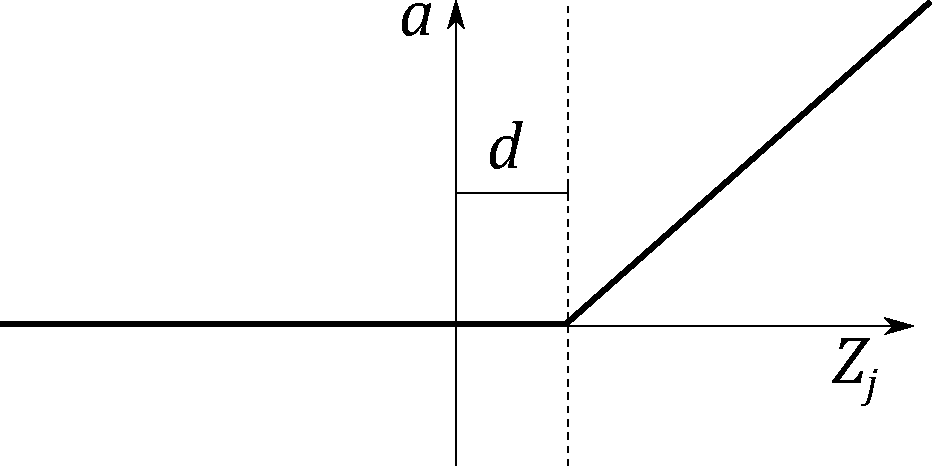
\includegraphics[width=0.5\linewidth]{images/relu.pdf}    

    \caption{In figure captions, explain what the reader is looking at: ``A schematic of the rectifying linear unit, where $a$ is the output amplitude,
    $d$ is a configurable dead-zone, and $Z_j$ is the input signal'', as well as why the reader is looking at this: 
    ``It is notable that there is no activation \emph{at all} below 0, which explains our initial results.'' 
    \textbf{Use vector image formats (.pdf) where possible}. Size figures appropriately, and do not make them over-large or too small to read.
    }

    % use the notation fig:name to cross reference a figure
    \label{fig:relu} 
\end{figure}


\begin{figure}
    \centering
    \begin{subfigure}[b]{0.45\textwidth}
        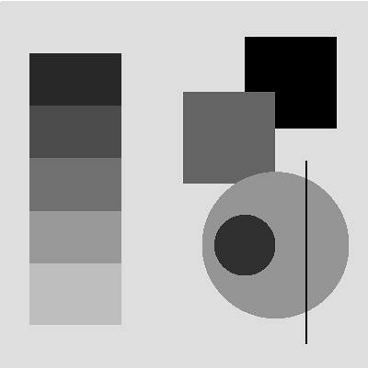
\includegraphics[width=\textwidth]{images/synthetic.png}
        \caption{Synthetic image, black on white.}
        \label{fig:syn1}
    \end{subfigure}
    ~ %add desired spacing between images, e. g. ~, \quad, \qquad, \hfill etc. 
      %(or a blank line to force the subfigure onto a new line)
    \begin{subfigure}[b]{0.45\textwidth}
        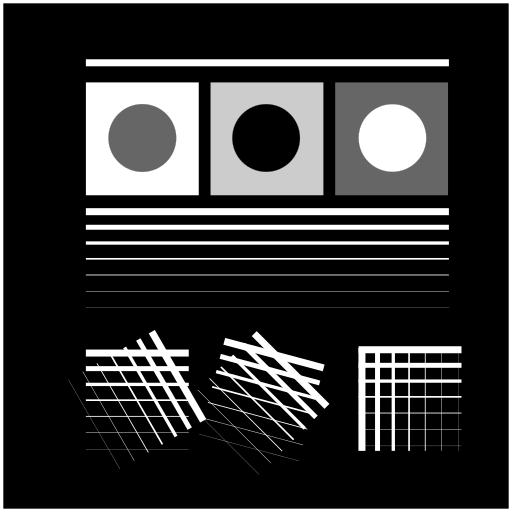
\includegraphics[width=\textwidth]{images/synthetic_2.png}
        \caption{Synthetic image, white on black.}
        \label{fig:syn2}
    \end{subfigure}
    ~ %add desired spacing between images, e. g. ~, \quad, \qquad, \hfill etc. 
    %(or a blank line to force the subfigure onto a new line)    
    \caption{Synthetic test images for edge detection algorithms. \subref{fig:syn1} shows various gray levels that require an adaptive algorithm. \subref{fig:syn2}
    shows more challenging edge detection tests that have crossing lines. Fusing these into full segments typically requires algorithms like the Hough transform.
    This is an example of using subfigures, with \texttt{subref}s in the caption.
    }\label{fig:synthetic}
\end{figure}

\clearpage

\subsection{Equations}

Equations should be typeset correctly and precisely. Make sure you get parenthesis sizing correct, and punctuate equations correctly 
(the comma is important and goes \textit{inside} the equation block). Explain any symbols used clearly if not defined earlier. 

For example, we might define:
\begin{equation}
    \hat{f}(\xi) = \frac{1}{2}\left[ \int_{-\infty}^{\infty} f(x) e^{2\pi i x \xi} \right],
\end{equation}    
where $\hat{f}(\xi)$ is the Fourier transform of the time domain signal $f(x)$.

\subsection{Algorithms}
Algorithms can be set using \texttt{algorithm2e}, as in Algorithm \ref{alg:metropolis}.

% NOTE: line ends are denoted by \; in algorithm2e
\begin{algorithm}
    \DontPrintSemicolon
    \KwData{$f_X(x)$, a probability density function returing the density at $x$.\; $\sigma$ a standard deviation specifying the spread of the proposal distribution.\;
    $x_0$, an initial starting condition.}
    \KwResult{$s=[x_1, x_2, \dots, x_n]$, $n$ samples approximately drawn from a distribution with PDF $f_X(x)$.}
    \Begin{
        $s \longleftarrow []$\;
        $p \longleftarrow f_X(x)$\;
        $i \longleftarrow 0$\;
        \While{$i < n$}
        {
            $x^\prime \longleftarrow \mathcal{N}(x, \sigma^2)$\;
            $p^\prime \longleftarrow f_X(x^\prime)$\;
            $a \longleftarrow \frac{p^\prime}{p}$\;
            $r \longleftarrow U(0,1)$\;
            \If{$r<a$}
            {
                $x \longleftarrow x^\prime$\;
                $p \longleftarrow f_X(x)$\;
                $i \longleftarrow i+1$\;
                append $x$ to $s$\;
            }
        }
    }
    
\caption{The Metropolis-Hastings MCMC algorithm for drawing samples from arbitrary probability distributions, 
specialised for normal proposal distributions $q(x^\prime|x) = \mathcal{N}(x, \sigma^2)$. The symmetry of the normal distribution means the acceptance rule takes the simplified form.}\label{alg:metropolis}
\end{algorithm}

\subsection{Tables}

If you need to include tables, like Table \ref{tab:operators}, use a tool like https://www.tablesgenerator.com/ to generate the table as it is
extremely tedious otherwise. 

\begin{table}[]
    \caption{The standard table of operators in Python, along with their functional equivalents from the \texttt{operator} package. Note that table
    captions go above the table, not below. Do not add additional rules/lines to tables. }\label{tab:operators}
    %\tt 
    \rowcolors{2}{}{gray!3}
    \begin{tabular}{@{}lll@{}}
    %\toprule
    \textbf{Operation}    & \textbf{Syntax}                & \textbf{Function}                            \\ %\midrule % optional rule for header
    Addition              & \texttt{a + b}                          & \texttt{add(a, b)}                                    \\
    Concatenation         & \texttt{seq1 + seq2}                    & \texttt{concat(seq1, seq2)}                           \\
    Containment Test      & \texttt{obj in seq}                     & \texttt{contains(seq, obj)}                           \\
    Division              & \texttt{a / b}                          & \texttt{div(a, b) }  \\
    Division              & \texttt{a / b}                          & \texttt{truediv(a, b) } \\
    Division              & \texttt{a // b}                         & \texttt{floordiv(a, b)}                               \\
    Bitwise And           & \texttt{a \& b}                         & \texttt{and\_(a, b)}                                  \\
    Bitwise Exclusive Or  & \texttt{a \textasciicircum b}           & \texttt{xor(a, b)}                                    \\
    Bitwise Inversion     & \texttt{$\sim$a}                        & \texttt{invert(a)}                                    \\
    Bitwise Or            & \texttt{a | b}                          & \texttt{or\_(a, b)}                                   \\
    Exponentiation        & \texttt{a ** b}                         & \texttt{pow(a, b)}                                    \\
    Identity              & \texttt{a is b}                         & \texttt{is\_(a, b)}                                   \\
    Identity              & \texttt{a is not b}                     & \texttt{is\_not(a, b)}                                \\
    Indexed Assignment    & \texttt{obj{[}k{]} = v}                 & \texttt{setitem(obj, k, v)}                           \\
    Indexed Deletion      & \texttt{del obj{[}k{]}}                 & \texttt{delitem(obj, k)}                              \\
    Indexing              & \texttt{obj{[}k{]}}                     & \texttt{getitem(obj, k)}                              \\
    Left Shift            & \texttt{a \textless{}\textless b}       & \texttt{lshift(a, b)}                                 \\
    Modulo                & \texttt{a \% b}                         & \texttt{mod(a, b)}                                    \\
    Multiplication        & \texttt{a * b}                          & \texttt{mul(a, b)}                                    \\
    Negation (Arithmetic) & \texttt{- a}                            & \texttt{neg(a)}                                       \\
    Negation (Logical)    & \texttt{not a}                          & \texttt{not\_(a)}                                     \\
    Positive              & \texttt{+ a}                            & \texttt{pos(a)}                                       \\
    Right Shift           & \texttt{a \textgreater{}\textgreater b} & \texttt{rshift(a, b)}                                 \\
    Sequence Repetition   & \texttt{seq * i}                        & \texttt{repeat(seq, i)}                               \\
    Slice Assignment      & \texttt{seq{[}i:j{]} = values}          & \texttt{setitem(seq, slice(i, j), values)}            \\
    Slice Deletion        & \texttt{del seq{[}i:j{]}}               & \texttt{delitem(seq, slice(i, j))}                    \\
    Slicing               & \texttt{seq{[}i:j{]}}                   & \texttt{getitem(seq, slice(i, j))}                    \\
    String Formatting     & \texttt{s \% obj}                       & \texttt{mod(s, obj)}                                  \\
    Subtraction           & \texttt{a - b}                          & \texttt{sub(a, b)}                                    \\
    Truth Test            & \texttt{obj}                            & \texttt{truth(obj)}                                   \\
    Ordering              & \texttt{a \textless b}                  & \texttt{lt(a, b)}                                     \\
    Ordering              & \texttt{a \textless{}= b}               & \texttt{le(a, b)}                                     \\
    % \bottomrule
    \end{tabular}
    \end{table}
\subsection{Code}

Avoid putting large blocks of code in the report (more than a page in one block, for example). Use syntax highlighting if possible, as in Listing \ref{lst:callahan}.

\begin{lstlisting}[language=python, float, caption={The algorithm for packing the $3\times 3$ outer-totalistic binary CA successor rule into a 
    $16\times 16\times 16\times 16$ 4 bit lookup table, running an equivalent, notionally 16-state $2\times 2$ CA.}, label=lst:callahan]
    def create_callahan_table(rule="b3s23"):
        """Generate the lookup table for the cells."""        
        s_table = np.zeros((16, 16, 16, 16), dtype=np.uint8)
        birth, survive = parse_rule(rule)

        # generate all 16 bit strings
        for iv in range(65536):
            bv = [(iv >> z) & 1 for z in range(16)]
            a, b, c, d, e, f, g, h, i, j, k, l, m, n, o, p = bv

            # compute next state of the inner 2x2
            nw = apply_rule(f, a, b, c, e, g, i, j, k)
            ne = apply_rule(g, b, c, d, f, h, j, k, l)
            sw = apply_rule(j, e, f, g, i, k, m, n, o)
            se = apply_rule(k, f, g, h, j, l, n, o, p)

            # compute the index of this 4x4
            nw_code = a | (b << 1) | (e << 2) | (f << 3)
            ne_code = c | (d << 1) | (g << 2) | (h << 3)
            sw_code = i | (j << 1) | (m << 2) | (n << 3)
            se_code = k | (l << 1) | (o << 2) | (p << 3)

            # compute the state for the 2x2
            next_code = nw | (ne << 1) | (sw << 2) | (se << 3)

            # get the 4x4 index, and write into the table
            s_table[nw_code, ne_code, sw_code, se_code] = next_code

        return s_table

\end{lstlisting}

%==================================================================================================================================
\chapter{Evaluation} 

Evaluation was carried to out to analyse if the program meets the functional and non-functional requirements discussed in the design section. Unit tests were created to ensure functional requirements of the program were meet. Angular end to end tests were made to test UI functionality while user evaluations were carried out to gain suggestions for improvements and feedback on ease of use of the application. Some suggestions have been added to the future work section while others are just discussed. 

\section{Unit Testing}
Unit tests were created with the Jasmine testing framework which came packaged with the Angular project. These tests were created to ensure that underlying code met the functional requirements and simulated the logic of the Turing Tumble as expected. These tests were also created to ensure that any refactoring undertaken had a safety net to ensure that no internal functionality was accidentally changed. Test coverage was calculated using the testing framework and is shown in the diagram \ref{fig:codeCoverage}. 

The diagram shows the statistics of the testing coverage provided by the unit tests. Classes were given the most comprehensive tests as they focused more on the underlying logic of the program and included aspects of the program that should never change, for example the logic of the pieces should always reflect the logic found in the physical Turing Tumble game. The test coverage for components was lower as the tests created did not cover all the UI elements that are displayed in the components HTML file. This was seen as acceptable as focus was given to testing the functionality for the program and less so on visual elements that would be displayed. In hindsight given the importance of creating an application that is visually appealing to users, more tests could have been created to ensure logic related to UI was under test. An overall statement coverage of 73\% was achieved showing that most aspects of the program were inspected and tested for correct functionality.

Important Unit tests that were created include
\begin{itemize}
    \item Connected GearBit components will have the same direction and all change when one is clicked.
    \item A user should be able to select a piece from the sidebar and then place this piece in a slot.
    \item The board should allow a marble to reach the bottom and then trigger the next coloured marble corresponding to the location that it lands in.
    \item When a new GearBit is connected to a set of GearBits it should change it's direction if required to ensure the set of GearBits all face the same direction.
    \item GearBits should marbles in the opposite direction to where they are facing and then should switch direction.
    \item Ramp pieces should send marbles in the direction they are facing.
    \item Crossover pieces should send marbles in the direction they are currently travelling.
    \item Bits should send marbles in the opposite direction to where they face, then change their direction.
    \item Interceptors should stop the marble travelling.
    \item PuzzleBoards should lock the starting pieces of a created puzzle when confirmed.
    \item The amount of marbles in a puzzle should only be increased if in the creation phase.
    \item Puzzles should update the number of pieces available correctly.
\end{itemize}

\section{UI Testing}
UI tests were created using the built in end to end testing framework 'Protractor'. This framework would allow certain DOM elements to be checked if visible and could allow simple button presses and router navigation. These tests would launch an instance of the site and travel through various pages by mimicking button presses. 

These tests ensured that the elements were still displayed correctly even when underlying component logic was changed or updated for example tutorial page information was still visible after adding a ta system. The tests were black box in style and didn't test underlying functionality only that the correct content was displayed to the user and that the user could navigate to the various pages. 

Test covered include 
\begin{itemize}
    \item A welcome message should be displayed to the user on the Home page.
    \item The side navigation bar should be opened and closed by the hamburger icon.
    \item A user should be able to select a piece to place on the board.
    \item The user should be able to navigate to the Tutorial page.
    \item The three separate tutorial sub sections should be visible.
    \item The theme of the program should be changeable by the user.
    \item A set of puzzles should be viewable when navigating to the Original Puzzles page. 
\end{itemize}

\section{Monitored User Tests}
Monitored user tests were carried to ensure that users could complete the tasks while having the option to ask for help or explanation if the tasks or site wasn't clear enough to use. The users were encouraged to give suggestions and improvements while working through the tasks and these were recorded. This allowed the user to give feedback on any aspect of the site, including aspects that were omitted from the evaluation form. 5 4th year Computer Science students were chosen for this test, this meant they should find the Turing Tumble game intuitive so would be able to focus on the websites ease of use instead of the games logic. The meetings were recorded so points made by the users can be recovered at a later date. The task sheet given to the users included 4 tasks and did not included a lot of detail or explanation of how to complete the tasks, for example they were asked to input a pattern without instruction to using the selection bar. This allowed for analysis to focus mainly on the ease of use that a user would have if they were to access the site separately and only have the tutorial to explain it's functionality. The tests took place over Zoom and the notes from these meetings can be found in the appendices.

\subsection{Task Explanation}
\label{taskExplanation}
Users were given an initial set up task followed by 4 tasks, one of which was optional

\begin{itemize}
    \item \emph{Task 0} - Asked the users the navigate to the tutorial page and spend some time reading the page giving basic details of the Turing Tumble game plus the functionality of the site.
    \item \emph{Task 1} - Asked the user to navigate to the plain board and add pieces to the board and walk through a basic Ramp pattern. They were then asked to experiment with the Bit and GearBit pieces. This allowed users to experience placing pieces and playing a Turing Tumble board. It also gave an opportunity to give the user an experience with the two of the more complicated pieces and focus on why they are important for the boards possible complexity.
    \item \emph{Task 2} - Asked the user open up the addition example and observe the addition ability of the board, they were also asked to experiment with the playback features. This gave the users the opportunity to see the more complicated patterns that can be made plus experience the playback features which they could later give feedback on.
    \item \emph{Task 3} - Asked the user to navigate to the Original Puzzles page and play with the difficulty filter, then to play through a puzzle. This allowed users to view the puzzle options on the site and evaluate playing through a puzzle.
    \item \emph{Task 4} - Was an optional task that asked users to create their own puzzle, using the Create Puzzle page. This allowed users to experiment with coming up and creating their own puzzle. This was given an optional as it could be difficult for people to come up with a puzzle for a game they have just experienced.
\end{itemize}

\subsection{Monitoring Session}
The user was asked to share their screen over a recorded Zoom call. They were told at the start of the meeting what was expected of them, including the ethics brief and how to contact me after the experiment. Notes were taken when a user asked questions or gave any suggestions. The number of times the user needed help was also recorded, for example one user didn't know how to change the direction of a piece. Other notes were taken of issues the user had that I observed when they carried out the tasks, for example one user didn't understand which part of the board would release the specific coloured marble.

\subsection{Evaluation Questions}
Users were given a variety of questions for each task. Initial questions gathered data on how many users were familiar with the Turing Tumble and how easy they found the initial task of placing pieces onto the board. They were asked at this stage if they had any suggestions to improve the previous task, focusing on how easy it was to place pieces and if the board gave enough detail to understand what was going on. Monitored users were also asked how easy they found GearBit pieces and if they have suggestions to improve their ease of use. Questions about Task 2 focused on if Bits could help improve their knowledge of registers in a CPU as well as if the playback features were easy to understand. Task 3 questions concerned how easy it was to select a puzzle and if they have any other suggestions for search or filter features. The final set of questions relating to the optional task asked users to evaluated how intuitive it was to create a puzzle and any suggestions they had to improve the experience. They were finally asked if they had any final suggestions for the program in general. A copy of the questions can be found in the appendices.

\subsection{Results}
The full list of responses given can be found in the appendices.

\emph{Task 1 questions}
2 out of the 5 users surveyed had heard of the Turing Tumble before, these users would be expected to find the program more intuitive than their peers as they have an expected idea of how the program should work compared to the physical board. All users found it easy to select and place pieces onto the board, this suggests that even though drag and drop may initially appear to be more intuitive, the users still found clicking and placing the pieces easy to use. 3 users did suggest a sort of highlighting system that would give feedback to the user if a piece could be placed on the slot they are hovering their cursor over. Users had no issues understanding that when a marble had 'fallen' off the board, this is likely due to the specific marble falling icon displayed. Most users had no issues changing the direction of a piece once placed but one suggested a tooltip to be placed on a piece to detail the that it can have it's direction changed by clicking. The users found that it wasn't entirely intuitive when two or more Gearbits were suggested, this is likely as there is no visible UI change when Gearbits are connected which all users suggested as an improvement. One user noted that the screen can be visually overwhelming and that a connection between the connected Gearbit can give a stronger intuition that they influence each other.

\emph{Task 2 questions}
The users agreed that the this task was somewhat helpful in improving understanding for how bits and registers work, this is understandable as the users were 4th year Computer Science students so will be expected to be very comfortable with these concepts. The piece icons were all found to be easily distinguished between each other, this is likely due to the strong colours which mimic the colours found in the physical Turing Tumble. Playback features were overall understood but a couple of the users suggested making them more clear and grouped together with the speed slider. This is maybe because all options related to the board are grouped together on the selection bar except the speed slider which is underneath the board. To improve understanding of the functionality of each piece, 3 users suggest a short clip or interactive tutorial giving examples of how the pieces interact with a marble. 

\emph{Task 3 questions}
Most users felt that the puzzle list was clear to showing the puzzles available, one didn't find it as clear as the others, a suggestion was given to implement an infinite scroll feature for the puzzles. All users agreed that the puzzle card displayed enough relevant information to help choose which puzzle to play. Some users found the difficulty filter useful while others not as much they suggested new filters based on the type of puzzle or a filter for puzzles that have already been completed. All users found it easy to understand the restrictions placed on a player and all agreed that they would help learn the various aspects of the Turing Tumble.

\emph{Task 4 questions}
All 5 users completed this extra task. They all found the starting phase easy to understand, this was likely due to the specific prompt displayed to the user for each phase of puzzle creation. One user didn't find puzzle creation easy when tasked with coming up with the solution after the starting set up and suggested that it may be easier to mark out the solution first then choose which of these pieces are part of the starting set up. The users suggested a few more descriptive attributes they would like added to their puzzles, some include the type of puzzle, a possible clear rate that could be calculated and having the difficulty replaced by the number of pieces a user would need to fill in to get the solution. 

\emph{Major suggestions during task and in evaluation response}
\label{suggestions}
\begin{itemize}
    \item The ability to reset the starting setup when creating a puzzle.
    \item Add an option for the board to automatically speed up when playing through a puzzle.
    \item Add an interactive tutorial.
    \item Let the user choose how many puzzles are displayed per page.
    \item Ghost image of a piece when hovering over a slot it can be placed in.
    \item A filter to show which direction each piece will send a marble.
    \item Add graphics to show when two or more Gearbits are connected via Gears.
    \item Add a small clip to explain what each piece does to a marble.
    \item Add a completed filter to the puzzle list.
    \item Search the puzzles by author.
    \item Filter the puzzles by the type of concept it implements.
    \item A keyword search on the puzzle description.
    \item Create puzzles by working from the solution then mark out which pieces are part of the starting set up.
    \item Give the clear rate of the puzzles.
\end{itemize}

\emph{Minor suggestions during task and in evaluation response}
\begin{itemize}
    \item Speed controls should be grouped with the rest of the playback options.
    \item Make the playback options a separate section.
    \item List of puzzles was initially only 5 so didn't look like the page was full, this was later updated to 10 puzzles per page to address this.
    \item Add tooltip detailing how to change the direction of a piece.
    \item Add exact speed data under the speed slider.
    \item Give some details of possible puzzle ideas when creating the puzzles.
    \item Example boards on main page should launch that example.
\end{itemize}

\emph{Notes taken while observing users}
\begin{itemize}
    \item One used wasn't exactly clear on the use of the reset marbles button compared to the reset board button. This is likely due to the buttons being very close in functionality, tooltips could maybe be added to give exact definitions for the buttons.
    \item Multiple users were confused with which marble would be triggered when it reached the bottom. A colour bar was added to help this but it doesn't seem to have helped make it more intuitive. More emphasis in the tutorial could be given to this or add some graphics to show the marble hitting a 'trigger' for another coloured marble.
    \item Some users were unaware of the tooltips for the pieces when hovered over so asked questions based on what each piece does. Could maybe add more information in the tutorial explaining this tool tip or have the currently held piece display it's tooltip in a prompt window. This would give the user clear instructions to what the piece does without the possibility of missing the information.
    \item One user found it difficult to find the different playback options as they didn't assume they would be in the same place as the selection bar. This could be improved by moving the playback options into their own separate bar. 
    \item A few users didn't initially see that the puzzle page had a paginator at the bottom so assumed that the 5 initial puzzles shown where the only ones available. This can be improved by adding an infinite scroll to get around the paginator or as a quicker fix the number of puzzles has been increased to have more of the page filled hopefully leading to the users eye spotting the paginator at the bottom.
    \item One user wasn't aware that the middle slot on the final row could send a marble to trigger the blue or red marbles. This could be fixed by including graphics that represent the physical board which could give a better intuition to this functionality.
    \item A user didn't initially known which side of the speed bar represented faster or slower. This could be made clearer by adding icons to represent an increase and decrease of speed.
    \item Some users tried to complete the puzzle by triggering a blue marble multiple times instead of once and letting the marbles to be spawn by the board. This could be more intuitive by only letting the user trigger the puzzle once unless they reset the marbles or board.
    \item One user was initially confused on how to change the direction of the piece and was looking for an option in the selection bar. This can be improved by one of their suggestions which was to add a tooltip over the piece which indicated that it can be switched direction. 
    \item One user was unsure of why the board was split into Pin slot and Component Slots. This was explained as a requirement in the physical board to allow the different pieces to stay in place. It may be beneficial to add this to the tutorial.  
    \item One user tried to drag and drop the pieces initially. This suggests that this may be the more intuitive option but they later found that the click and place was more effective for large quantity of pieces.
    \item One user made a mistake while creating the starting pieces for their puzzles and tried to go back but was unable. This could be added as a feature. 
    \item One user wasn't clear that the solution for a created puzzle must be generated by playing through the puzzle that was made. More emphasis can be given to this in the tutorial and prompt the user gets while on this stage.
\end{itemize}

\subsection{Limitations}
The monitored study was conducted remotely due to the ongoing COVID-19 pandemic. While the remote survey still provided valuable feedback from the users it would have been preferable to conduct the study in person to make the experience less rigid as the recorded zoom call had a more formal approach which in some cases lead to some users not speaking out as much as they may have done in person. While not the ideal environment this remote approach was seen as acceptable given the current environment.

The users of this study were all 4th Computer Science students. While they come under the target audience of this program as they have a clear interest in computing, I would have preferred to have had a greater share school pupils beginning their studies in computer science as the main target for thi survey. It would have been valuable to gain more feedback from this demographic as one of the main objectives of the program is to be useable and enjoyable replacement for a physical Turing Tumble in a class room. 

The main focus of this task was to gain feedback on the ease of use of the program. Ideally the program could be used in multiple sessions to gain more feedback of using the program as would in a possible class environment where pupils are encouraged to use the site and work through all the puzzles as part of their learning experience. This was seen as okay given the inability to ask pupils to evaluate the site over long period of time so only 2 questions were concerned with if the site could be useful for learning. 

While the users were given some time at the start of the study to read the tutorial it was noted by some users that it was a lot of information to take in before starting the study. This lead to a few scenarios of users not understanding the logic behind the Turing Tumble board game itself as they struggled to remember all the rules of the game from the tutorial. This lead to some issues with how various pieces worked which slowed down the progress of some users leading to questions and suggestions being added more about the game itself than how the program was performing. This was deemed an acceptable risk as an interactive tutorial, which would likely convey the information needed to use the site in an easier to understand manner, was seen as a feature outside the scope of the program. 

Some users were more willing to ask for help than others. It was unclear if these users were more interested in learning the inner workings of the program instead of trying to work out how to use the site intuitively. This may have lead some users to asking more help than they actually required to complete the task instead of reading the task sheet again. For 2 users it was deemed necessary to give help when they were undertaking the puzzle task incorrectly, this was noted down as the user needing help even thought they did not ask for it. It was decided that the user didn't want to be seen to be failing the puzzle so was more reluctant to ask for help or re-read the task sheet.  


\section{Unmonitored User Evaluations}
The unmonitored user evaluations were given out after the user returned a sign consent form, which can be found in the appendices. The user was given the ethics brief and was then sent a task sheet giving the details of how to access the site, the task specifications plus a link to the Google form used for the evaluation questions. A mix of 4th Computer Science students and school pupils undertaking Computer Science studies in school were chosen. Both groups were seen as the target demographic as they have a keen interest in the field and would have valuable feedback to the usability of the program. This task was seen as a more realistic evaluation of how many users would use the site as they would only have the tutorial page to understand the functionality of the program with no help on hand. The task sheet was designed to focus on giving only as much information as required to complete the tasks, with a focus on using the tutorial page, not the task sheet, to learn how to use the program. This was seen as a more realistic evaluation of how many users would use the site, leading to more responses based on how easy the site was to use not based on how well the task sheet give them instructions.

\subsection{Task Specification}
The task specifications for the unmonitored user evaluation follows very closely the tasks given in section \nameref{taskExplanation}. With the only major difference was the removal of the section of using Gearbits. This section of the task sheet was deemed too complex for a task sheet explanation and was left in the monitored evaluation as more information could be given as to why the Gearbits were important and could be used to make the board Turing complete. The task specification can be found in the appendices.

\subsection{Evaluation Questions}
Users were given a variety of questions for each task. The questions given to the unmonitored users were identical to the questions given to the monitored user evaluations however the questions concerning the Gearbits were removed. The evaluation questions can be found in the appendices. 

\subsection{Results}
The full list of responses given can be found in the appendices.

\emph{Task 1 questions}
Of the 7 responses given, no users had previously heard of the Turing Tumble game before accessing the site. This lead to evaluations that focused purely on the ease of use of the program and how intuitive it was to understand the logic of the game without a understanding of the physical game to compare to. All users found it easy to select and place pieces onto the board but suggestions were given to include a drag and drop feature as this was seen as more intuitive. This suggests that even though a drag and drop feature may be initially more intuitive they found the click place equally as easy to use. Most users found it easy to understand when a marble 'fell' off the board but a few users found this not understandable at all, suggesting that an animation should be added to give a clearer representation of the marble falling. This suggestions that the icon given to the marble falling is suitable for some but not all, possible improvements to this could be deemed as future work. All but one of the users found the pieces easy to change direction but one suggested that a hint should be given that clicking on a piece changes it direction. This suggests that while most found it easy to understand that clicking a piece changed its direction but that a graphical hint could be added to eliminate any possible confusion.

\emph{Task 2 questions}
Half of the users surveyed responded that the addition example was somewhat helpful in explaining the concepts of bits and registers with saying it definitely helped with one user saying it didn't. This suggests that if more the Turing Tumble board could be helpful in teaching some concepts of Computer Science but more focus should be given on learning using the site but possibly adding a learning section to the site. All users found it easy to uniquely identify the pieces, this suggests that no issues were found determining the different pieces by their individual icons. Most users found no issues understanding the different playback features of the site but one user found it harder than the rest, this suggests that tooltips could be added to the buttons to give a brief sentence of what they do when hoovered over.   

\emph{Task 3 questions}
All users found the puzzle suitably clear to use, with only one suggesting that by having only 5 puzzles on the page it wasn't clear there was a paginator at the bottom that would go through the rest of the list. This suggest that 5 puzzles per page was too small for a clear list, this was refactored to 10 to improve visibility. All users found that the information given in the puzzle tabs were relevant in choosing a puzzle. This suggests that the tab system that gave all the information that the physical version of the Turing Tumble puzzles give is enough to be confident of what a puzzle will entail. Most users found the difficulty filter useful but suggestions were given for different filters. The difficulty filter was overall seen as useful but future work could difficulty be added to add new filters or search features to make the finding a new puzzle easy and intuitive. Most users found that the starting set up pieces that couldn't be edited were clear however 2 users didn't find it very clear. This suggests that while the tutorial explains they can't be changed a icon could maybe be added when hovering over a locked piece to improve understanding. All users found it easier to understand the number of pieces they had to complete the puzzle. This suggests that the number denoting the pieces left to use next to the piece icon is suitable to convey the number of pieces available. One user detailed an issue they had were they tried to click the 'default puzzles' link when playing a puzzle to go back before finding the 'go home' button on this page. By clicking the link to a component they are already viewing it doesn't update the page when clicking the link, this could be improved by making the 'go home' button more clear or looking into ways have the links reload the current component a user is viewing.

\emph{Task 4 questions}
Only 3 users chose to complete the final optional task. All users found it clear to create the starting set up phase. This suggests that the tutorial and the prompt given to the user was clear enough to understand what phase they were creating. The users were split on if it was easy to come up with a solution by thinking of the solution to a possible puzzle. This suggests that the design requiring a user to come up with a solution to the puzzle they make may not be the most intuitive when it comes to creation, future work can be seen as designing a possible replacement for this feature. Some suggestions given for this include creating a pattern on the board then marking out which parts would be the starting slots in a puzzle.

\emph{Major unique suggestions given in unmonitored evaluation response}
\begin{itemize}
    \item Adding a hint descriptive feature when creating a puzzle.
    \item The ability to create puzzles by using a coding style text input.
    \item Add an animation of the marble dropping out of the board to indicate when it fell.
\end{itemize}

\emph{Minor suggestions given in unmonitored evaluation response}
\begin{itemize}
    \item Make the collected marbles component responsive to the screen size.
\end{itemize}

Other suggestions were given but were previously covered by the monitored evaluation responses in section \nameref{suggestions}.

\subsection{Limitations}
One limitation of the unmonitored survey is that the number of responses given does equate to the number of signed consent forms returned so some users may have looked at the site and decided against the tasks possibly due to initial information overload that the tutorial may not have helped explain. These views would have been useful to gain when evaluating the program.

6 responses were gained for the evaluation survey. While valuable information was obtained the number of responses from school pupils was low (1), which is unavoidable given the current pandemic and the inability to go into a school and help explain the tasks and give more motivation for the pupils to give feedback. This feedback would have been insightful as possible future work could be focused on making the program as easy to use and fun as possible for a school environment. 

The survey took around 30 minutes to complete yet it still missed some features I would have liked to have tested given more time but I decided to keep the tasks shorter to ensure I didn't lose the attention of the participant. More tasks related to learning via the program would have been desireable but as 50\% of participants didn't complete the last optional task, any more tasks or questions would have likely been too many and wouldn't have gathered much useful feedback.

\subsection{Discussion on given suggestions}
% This will likely be cut as it isn't work I did so doesn't matter
This section discuses some of the major suggestions given by users and if they should be detailed in the future work section or if they shouldn't be focused on given the scope of this project.

\emph{Interactive tutorial}
This suggest was one of the more common given across both groups of participants. This suggestion was considered during development but wasn't given enough development time to create this feature, it was decided that time should be more spent on making the more logic based features of the application strong, particularly the puzzle making and playing instead of focusing on a feature rich tutorial that would be used by a user one or two times at most. This feature would certainly help reduce the information overload experienced by some users and help give exact examples for how each piece works another common issue raised. Given more time with the project an interactive tutorial would be a strong feature that could help reduce confusion with the program and Turing Tumble board itself. 

\emph{Automatically speed up board while playing puzzles}
This suggestion involves having the speed slider increase after a few marbles have been collected while a puzzle is in play. This suggestion goes against the idea that the users should have total control of all aspects when it comes to the board and it was decided that the speed should only ever be controlled by a user so they can control which speed helps them understand the board the easist.

\emph{Choose how may puzzles are displayed}
This suggestion as given by multiple users and aimed to sort the problem of the puzzle page looking half full leading to some users not noticing that their was a page system for the puzzles. This could be classified as future work but for an initial improvement the number of puzzles per page has been increased to 10. This makes the page full hopefully addressing the issue of some users not seeing the page system at the bottom as the list won't know give the impression of only being half full.

\emph{Ghost Image when hovering over a slot}
This suggestion was given by multiple users and entails a opaque icon of the currently held piece to be displayed when hovered over a valid slot. This suggestion will be added to the list of future work as it should reduce any possible confusion of how to place pieces into the board. This wasn't a particularly common issue found by users but as it is one of the most fundament functions of the board, it is important that it is as easy to use as possible.

\emph{A filter to show direction marble would travel}
A user suggested this during a monitored evaluation as a way to understand in more basic terms what each component would do upon reaching a marble. This will not get added to future work as one of the important aspects of understanding the Turing Tumble is either working out the flow of the marble by tracing the path with the a finger or by playing the marble and noticing where it goes. TO most accurately capture the physical board I think it's important to encourage either of these two methods, by adding this filter it may encourage users to look at what the filter would tell them would happen instead playing it out themselves which can seen as a valuable way to learn the game.

\emph{Graphics to show when multiple Gearbits are connected}
This suggestion was the most prevalent from the monitored responses. The users found it difficult to intuitively understand that Gearbits connected via Gears influenced each other when clicked. They suggested that a graphical line connecting the pieces together could help imply the connection that they have. This is one of the most useful suggestions given as the Gearbit is one of the most important pieces for the game and any way to improve the understandability of the piece would encourage more use of it in puzzles or examples increasing the learning impact it could have. This will definitely been seen as future work.

\emph{Add a clip explaining the use of each piece}
This suggestion can be seen as a smaller solution compared to an interactive tutorial and work could be added to record some some video clips giving an example of each pieces use in the board context. This feature along could help resolve a lot of the understanding issues that some users had while going through the puzzles and could help solve it. This feature could also be implemented as part of an interactive tutorial and will be included in future work as any feature that improves the usability of the program will help encourage more people to return and learn using the board.

\emph{Add a completed filter to the puzzle list}
This feature could only be implemented if a user was to login, at that stage the site could look to store data based on the users interactions with the site. This filter could encourage people to go through all the default puzzles and ensure they complete them in order or at least have a go at each puzzle. As this is the main way to learn the board it may be a good feature to add to encourage this behaviour. 

\emph{Search the puzzle by author}
Another feature that was suggested by one of the users was the ability to filter the puzzles by the author that created them. This feature could be added if the user section of the site continued to grow and a large body of puzzles was made by unique users to justify this feature. It can be considered a future work feature but only after the user part of the site is fleshed out in areas. This may encourage more user puzzles and a sense of pride in making the puzzle if other users can be encouraged to search for puzzles by their favourite authors.

\emph{Filter the puzzles by type of concept that the puzzle implements}
Another search feature suggested by some users was to give tags to the puzzles which could give information based on the type of puzzle they are. Examples given by users would be addition or puzzles. More tags could be created for the site or user custom tags could be looked in to. This feature will be included into the future work as it gives another descriptive feature to the puzzles as well as adding another search feature for the user. 

\emph{Search the puzzles by searching for terms that appear in the description}
This search could added in future work as another search function to improve how easy it is for users to search and find different puzzles they wish to play. The only issue with this search feature is focusing on the description of a puzzle made by a user which may not be the most accurate description of a puzzle. It can be included as part of a possible future work that focuses on improving the search features for the puzzle list.

\emph{Mark out the starting pieces after creating the solution}
This suggestion was given by a user to change the way puzzles are created, they suggest that it is more intuitive to create a puzzle by making the pattern first then marking out which pieces are the starting set up. This can be added but as only one user suggested this it would be important to conduct another user survey to see if this method would be more preferable.

\emph{Give the clear rate of puzzles}
This feature can be added once the user section of the page is giving more features and data about the user's completion rate of a puzzle is added. The solution to puzzles would also need to be removed to reduce people looking at the solution then completing the puzzle afterwards to give the impression they had completed the puzzle. This could be added to future work but isn't the most common filter feature suggested by users.

\emph{Adding a hint descriptive feature to the puzzle creation}
One user suggested that a hint descriptive element can be added to a puzzle the user creates. This hint could then be shown to a user instead of showing them the solution set up. This feature in combination with previous suggestions about clear rate or filter on user's completing puzzles could be used to give greater control to a user's search. This can be seen as a replacement to the solution set of the puzzle object and could be seen as a possible replacement for the current feature of showing the user the solution.

\emph{The ability to create puzzles by using a coding style input}
This feature was suggested as a possible change to the current puzzle creation feature. This will not be put under future work, while the suggestion is novel and interesting it is far outside the scope of the project and the possible advantage of this implementation over using the current method could involve speed but the learning curve for this feature and the server side code needed to work out what puzzle they were creating wouldn't be worth the development effort for the average user.

\emph{Animation for the marble falling off the screen}
One user suggested adding an animation to indicate when the marble had fallen. This would likely eliminate any confusion that could be had of what happens when a ball reaches an empty slot on the board. Animation for the board in whole is part of the future work section and this suggestion could be added as part of it.

\subsection{Issues known about the program}
\begin{itemize}
    \item The current program is not responsible on a mobile browser. This was known during the design and implementation of the program. To make the program responsive for a mobile device, the front end code focusing on how the elements display to the page would require a different library to give different sizes to different elements based on the type of device the program is currently displayed on. This was seen as something outwith the scope of the project as it was decided at the design stage that it was primarily focused on displaying information on a desktop browser. The site currently breaks when viewed on a mobile phone and some of the most fundamental features of the program no longer work, for example a user can not place a piece on the board correctly as the board is pushed off the screen.
    \item The program sends the puzzle data to the backend firebase server by converting the puzzle object to JSON representation then saving this file in the server. This method was chosen to focus on getting the data stored correctly and then spending more development time on the user facing features of puzzle creation and playing. A single default puzzle is 19.8 kB large when stored on the server. A fix to this would be remove the current implementation of sending up the entire puzzle object and instead only send up the details of changes and important data for example instead of sending up the list of slots for the set up and solution slot lists. A single JSON file can be made that details where pieces are located for each set up instead of sending up data about the board that is already known for example the number of Pin and Component Slots stored in a board object. This issue is something that would improve the backend performance for the site and would lead to a more efficient program. 
    \item As noted by some users during the monitored evaluations, some aspects of the site on desktop are not fully responsive meaning they can reduce the width of the screen while on a plain board and the selection bar will become hidden behind the board which won't change it's width. This issue was known while creating the site and focus was given to the pages being fully visible with no data being hidden lower on the page, requiring no scrolling from the user. As future work, responsive front end logic should be added so that the board and selection bar don't overlap on each over, this would improve ease of use and usability for a desktop user.
    \item Full animation of the board involving gravity was explored as a possible avenue for design. It was decided early on that more focus should be given towards creating a puzzle environment for users and then spending any extra development time on full animation after the main requirements were met. Full animation is a desired function to greatly improve user feedback and help aid understanding of the board while in play. Future work could be to implement this feature into the site. One issue with the current design of the program leads to a focus on having a collection of small modular component each with it's own HTML elements. This doesn't lead naturally to the extension of using an external physics library as a lot of code would need to be changed to deal with the logic of gravity and the api calls to the external library. It will still be included in future work but it is important to evaluate the design of the program doesn't lead itself naturally to this new feature.   
\end{itemize}

\subsection{Program efficiency via lighthouse}
To evaluate the perform efficiency and performance. Lighthouse (REF) was used to generate a report on the performance, accessibly and best practices used on each page. The report also gave suggestions to why some metrics may be lower than other plus suggestions to improve them. The overall scores for 4 pages are shown in \ref{tab:lighthouse}. The testing was performed using the Lighthouse CLI tool while the page was hosted on the main development machine. 

\begin{table}[]
    \caption{The table of lighthouse metric scores for 4 pages of the program.}\label{tab:lighthouse}
    \begin{tabular}{llllll}
    Page            & Performance & Accessibility & Best Practices & Speed Index & Largest Contentful Paint \\
    Home            & 39          & 100           & 93             & 4.2s        & 5.7s                     \\
    Plain Board     & 51          & 87            & 93             & 4.1s        & 5.4s                     \\
    Tutorial        & 60          & 96            & 93             & 4.1s        & 4.7s                     \\
    Default Puzzles & 51          & 98            & 93             & 4.1s        & 4.6s                    
    \end{tabular}
    \end{table}

As shown from the metrics above the performance was acceptable for most pages but not high enough overall to meet the non-functional requirement (PUT REQ HERE). Suggestions from the lighthouse tool include removing unnecessary JS from the first load. This is due to the design of the routing functionality of the program. The home page will load all pages can access before displaying it's own content. This is down to the router functionality where it ensures all components it can route to are sent to the users client before they can access those links. Future work can be given to improve the performance metrics of this program. While not meeting the non-functional requirement for strong performance, a focus on the features available for the users was seen as an acceptable compromise to diverting development time towards performance metrics. 

The Home and Plain Board pages were shown to have the longest Largest Contentful Paint time, this metric describes the time taken to display the largest text or graphic content on the page. Both pages include large amounts of data to display the board with all it's icons and Board parts i.e. 4 example boards on the Home page. Other suggestions to improve performance across all pages was to reduce the DOM size, this is down to the high modulation of components that was chosen for the design leading to large list of HTML components on most pages. This wss seen as an acceptable compromise as high component design reduced repeated code during development and allowed for greater abstraction. Future work can be given to explore avenues to improve these performance metrics across all pages taking note of the opportunities identify by lighthouse as well as focusing on minimise component size and cutting down on unnecessary DOM size.   

\section{Overall}
\subsection{Talk about how it meets functional reqs}
\subsection{Talk about how it meets non-functional reqs or moscow}




\begin{figure}
    \centering
    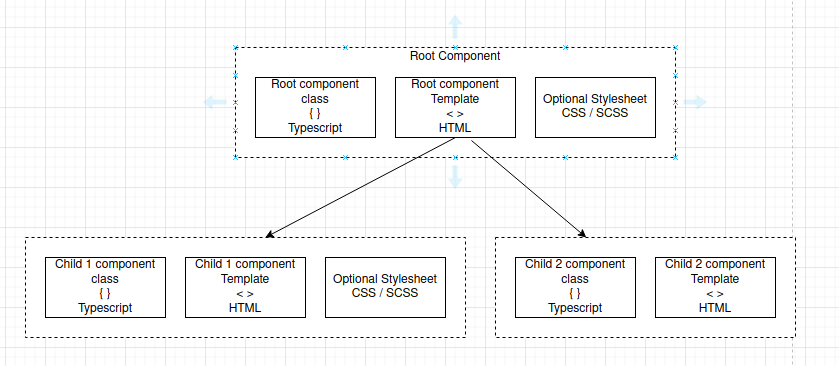
\includegraphics[width=1\linewidth]{images/codeCoverage.png}    

    \caption{ This code coverage table was produced by the testing framework and shows the test coverage for different parts of the program including the typescript classes and Angular components created. 
    }

    % use the notation fig:name to cross reference a figure
    \label{fig:codeCoverage} 
\end{figure}

How good is your solution? How well did you solve the general problem, and what evidence do you have to support that?

\section{Guidance}
\begin{itemize}
    \item
        Ask specific questions that address the general problem.
    \item
        Answer them with precise evidence (graphs, numbers, statistical
        analysis, qualitative analysis).
    \item
        Be fair and be scientific.
    \item
        The key thing is to show that you know how to evaluate your work, not
        that your work is the most amazing product ever.
\end{itemize}

\section{Evidence}





Make sure you present your evidence well. Use appropriate visualisations, reporting techniques and statistical analysis, as appropriate.

If you visualise, follow the basic rules, as illustrated in Figure \ref{fig:boxplot}:
\begin{itemize}
\item Label everything correctly (axis, title, units).
\item Caption thoroughly.
\item Reference in text.
\item \textbf{Include appropriate display of uncertainty (e.g. error bars, Box plot)}
\item Minimize clutter.
\end{itemize}

See the file \texttt{guide\_to\_visualising.pdf} for further information and guidance.

\begin{figure}
    \centering
    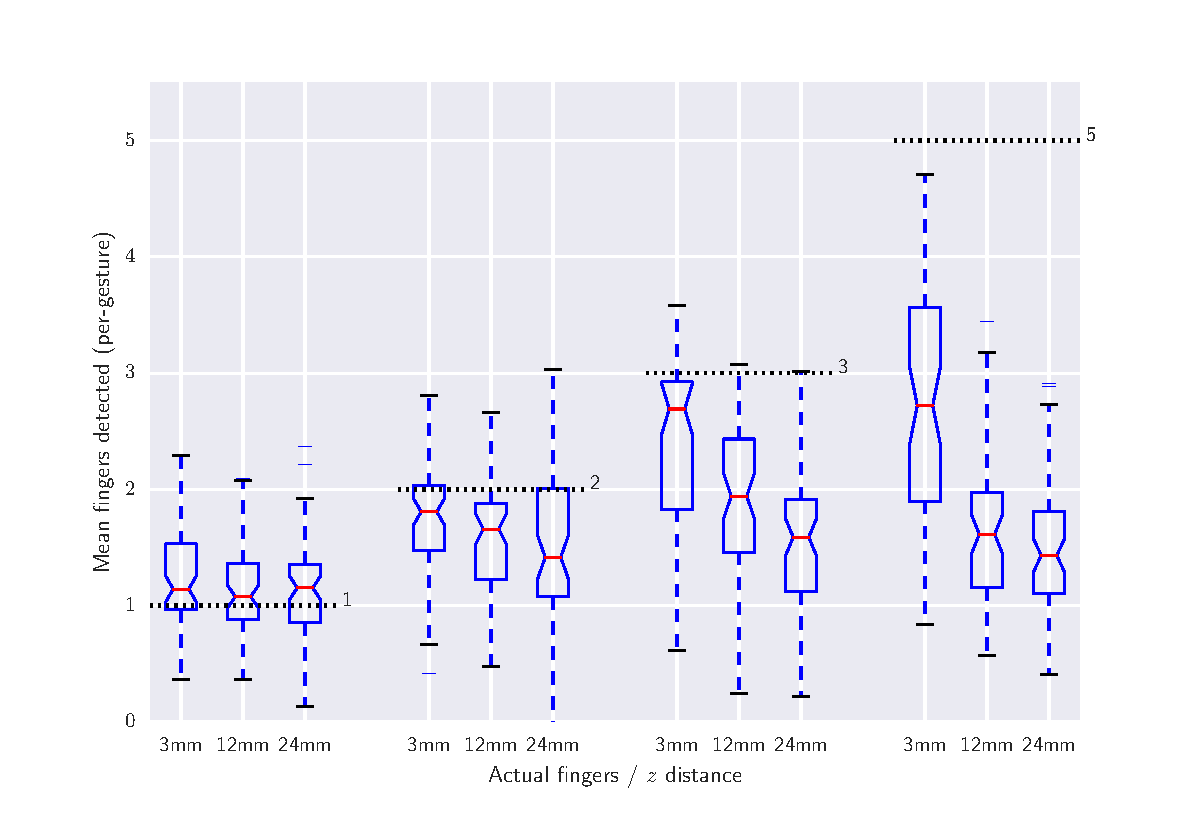
\includegraphics[width=1.0\linewidth]{images/boxplot_finger_distance.pdf}    

    \caption{Average number of fingers detected by the touch sensor at different heights above the surface, averaged over all gestures. Dashed lines indicate
    the true number of fingers present. The Box plots include bootstrapped uncertainty notches for the median. It is clear that the device is biased toward 
    undercounting fingers, particularly at higher $z$ distances.
    }

    % use the notation fig:name to cross reference a figure
    \label{fig:boxplot} 
\end{figure}


%==================================================================================================================================
\chapter{Conclusion}    
Summarise the whole project for a lazy reader who didn't read the rest (e.g. a prize-awarding committee).
\section{Guidance}
\begin{itemize}
    \item
        Summarise briefly and fairly.
    \item
        You should be addressing the general problem you introduced in the
        Introduction.        
    \item
        Include summary of concrete results (``the new compiler ran 2x
        faster'')
    \item
        Indicate what future work could be done, but remember: \textbf{you
        won't get credit for things you haven't done}.
\end{itemize}

%==================================================================================================================================
%
% 
%==================================================================================================================================
%  APPENDICES  

\begin{appendices}

\chapter{Appendices}

Typical inclusions in the appendices are:

\begin{itemize}
\item
  Copies of ethics approvals (required if obtained)
\item
  Copies of questionnaires etc. used to gather data from subjects.
\item
  Extensive tables or figures that are too bulky to fit in the main body of
  the report, particularly ones that are repetitive and summarised in the body.

\item Outline of the source code (e.g. directory structure), or other architecture documentation like class diagrams.

\item User manuals, and any guides to starting/running the software.

\end{itemize}

\textbf{Don't include your source code in the appendices}. It will be
submitted separately.

\end{appendices}

%==================================================================================================================================
%   BIBLIOGRAPHY   

% The bibliography style is abbrvnat
% The bibliography always appears last, after the appendices.

\bibliographystyle{abbrvnat}

\bibliography{l4proj}

\end{document}
